\documentclass[a4paper,12pt]{report}

% ============================================================
% PACKAGES
% ============================================================
\usepackage[utf8]{inputenc}
\usepackage[T1]{fontenc}
\usepackage{lmodern}
\usepackage[english]{babel}
\usepackage[margin=2.5cm]{geometry}
\setlength{\headheight}{14.5pt}
\addtolength{\topmargin}{-2.5pt}
\usepackage{graphicx}
\usepackage{xcolor}
\usepackage{titlesec}
\usepackage{fancyhdr}
\usepackage[pdftex]{hyperref}
\usepackage{setspace}
\usepackage{parskip}
\usepackage{booktabs}
\usepackage{longtable}
\usepackage{array}
\usepackage{multirow}
\usepackage{tabularx}
\usepackage{float}
\usepackage{caption}
\usepackage{subcaption}
\usepackage{amsmath}
\usepackage{amssymb}
\usepackage{enumitem}
\usepackage{listings}
\usepackage{tikz}
\usetikzlibrary{arrows.meta, positioning}
\usepackage{tocloft}

% ============================================================
% CONFIGURATION
% ============================================================
\hypersetup{
    colorlinks=true,
    linkcolor=black,
    urlcolor=blue,
    citecolor=black
}

\onehalfspacing

% Chapter title formatting
\titleformat{\chapter}[display]
    {\normalfont\huge\bfseries}
    {\chaptertitlename\ \thechapter}{20pt}{\Huge}
\titlespacing*{\chapter}{0pt}{-20pt}{40pt}

% Header/footer
\pagestyle{fancy}
\fancyhf{}
\fancyhead[L]{\leftmark}
\fancyhead[R]{\thepage}
\renewcommand{\headrulewidth}{0.4pt}
\fancypagestyle{plain}{
    \fancyhf{}
    \fancyfoot[C]{\thepage}
    \renewcommand{\headrulewidth}{0pt}
}

% Code listing style
\lstset{
    basicstyle=\ttfamily\small,
    backgroundcolor=\color{gray!10},
    frame=single,
    framerule=0pt,
    breaklines=true,
    captionpos=b
}

\begin{document}

% ============================================================
% COVER PAGE
% ============================================================
\begin{titlepage}
    \begin{center}
        
        % --- Top logos row ---
        \begin{minipage}{0.3\textwidth}
            \centering
            
\includegraphics[height=2cm]{logos/fst_logo.png}
        \end{minipage}
        \hfill
        \begin{minipage}{0.3\textwidth}
            \centering
            
\includegraphics[height=2cm]{logos/manar_logo.png}
        \end{minipage}
        
        \vspace{0.2cm}
        \rule{\textwidth}{1pt}
        
        \vspace{0.5cm}
        
        % --- Department and report type ---
        {\large \textbf{Computer Science Department}}\\[0.2cm]
        {\Large \textbf{Summer Internship Report}}\\[0.2cm]
        {\large Second Year in Software Engineering}\\[0.5cm]
        
        % --- Author ---
        {\large Presented by: \textbf{Yassine Ben Jemaa}}\\[0.8cm]
        
        % --- Title ---
        \rule{0.8\textwidth}{0.5pt}\\[0.3cm]
        {\LARGE \textbf{Design and Implementation of a\\[0.2cm]
        Real-Time Anomaly Detection Platform\\[0.2cm]
        for Branch Teller Operations\\[0.2cm]
        using Deep Learning}}\\[0.3cm]
        \rule{0.8\textwidth}{0.5pt}\\[0.8cm]
        
        % --- Supervisor ---
        {\large Supervisor: \textbf{Mr. Oussama Ben Cheikh}}\\[0.5cm]
        
        % --- Company ---
        {\large Realized within:}\\[0.3cm]
        
\includegraphics[height=2cm]{logos/amen_logo.jpeg}\\[0.8cm]
        
        % --- Academic year ---
        {\large \textbf{Academic Year: 2025--2026}}
        
        \vfill
        
        % --- Bottom bar ---
        \rule{\textwidth}{1pt}\\[0.2cm]
        \begin{minipage}{0.45\textwidth}
            \small
            Faculté des Sciences de Tunis\\
            Université de Tunis El Manar\\
            2092 El Manar, Tunis
        \end{minipage}
        \hfill
        \begin{minipage}{0.45\textwidth}
            \raggedleft\small
            \url{www.fst.rnu.tn}
        \end{minipage}
        
    \end{center}
\end{titlepage}

% ============================================================
% FRONT MATTER
% ============================================================
\pagenumbering{roman}

% --- Acknowledgements ---
\chapter*{Acknowledgements}
\addcontentsline{toc}{chapter}{Acknowledgements}

I would like to express my sincere gratitude to Amen Bank for offering
me the opportunity to complete this internship within the Direction
Centrale du Système d'Information. I would especially like to thank
my supervisor, Mr.\ Oussama Ben Cheikh, for his guidance and for
granting me the freedom to explore beyond the original project scope.

This experience allowed me to acquire practical skills in deep learning,
streaming architectures, and MLOps, and to discover the challenges of
building production-oriented systems in a real banking environment.

I would also like to thank the Faculté des Sciences de Tunis and the
University of Tunis El Manar for the academic foundation that made
this work possible.

\newpage

% --- Table of Contents ---
\tableofcontents
\newpage

% --- List of Figures ---
\listoffigures
\addcontentsline{toc}{chapter}{List of Figures}
\newpage

% --- List of Tables ---
\listoftables
\addcontentsline{toc}{chapter}{List of Tables}
\newpage

% --- List of Abbreviations ---
\chapter*{List of Abbreviations}
\addcontentsline{toc}{chapter}{List of Abbreviations}

\begin{tabular}{@{}ll@{}}
    AE       & Autoencoder \\
    AML      & Anti-Money Laundering \\
    AUC      & Area Under the Curve \\
    BCT      & Banque Centrale de Tunisie \\
    CTAF     & Commission Tunisienne des Analyses Financières \\
    DI       & Dependency Injection \\
    DLQ      & Dead Letter Queue \\
    DT       & Dinar Tunisien \\
    E2E      & End-to-End \\
    FK       & Foreign Key \\
    FT       & Financing of Terrorism \\
    KPI      & Key Performance Indicator \\
    LAB      & Lutte Anti-Blanchiment \\
    LSTM     & Long Short-Term Memory \\
    MLOps    & Machine Learning Operations \\
    NLG      & Natural Language Generation \\
    ROC      & Receiver Operating Characteristic \\
    SHAP     & SHapley Additive exPlanations \\
\end{tabular}

\newpage

% ============================================================
% MAIN CONTENT
% ============================================================
\pagenumbering{arabic}

% --- Introduction ---
\chapter*{General Introduction}
\addcontentsline{toc}{chapter}{General Introduction}
The digital transformation of retail banking has shifted the volume and
velocity of financial transactions well beyond what manual oversight can
monitor. In a network of 150 branches processing thousands of teller
operations daily, the gap between transaction speed and supervisory
capacity creates exposure to fraud, money laundering, operational errors,
and behavioral anomalies that may go undetected until periodic compliance
reviews surface them --- often weeks or months after the fact.

Amen Bank's Direction Centrale du Système d'Information already operates
an AI-based anti-money laundering system oriented toward bank-wide
compliance reporting. This internship addresses a complementary need:
real-time decision support for branch supervisors at the point of
transaction. The objective is to design and build a platform that ingests
teller operations as they occur, profiles both the client and the
employee involved, detects anomalies using deep learning models, and
surfaces explainable alerts that a non-technical supervisor can
understand and act upon immediately.

The platform covers four teller-window operations --- retrait, versement,
virement, and remise de chèques --- and monitors two independent actors
per transaction: the client initiating it and the employee processing it.
An Autoencoder detects point anomalies in individual transactions while
an LSTM network identifies sequential deviations in client behavior over
time. Every alert is accompanied by a human-readable explanation
generated through SHAP, bridging the gap between model output and
supervisory action.

Beyond the detection models themselves, the project invests in the
infrastructure that makes a machine learning system operational and
maintainable: a streaming pipeline built on RedPanda, behavioral
profiles maintained through a hot/cold data layer, automated experiment
tracking with MLflow, three independent retraining triggers, structured
logging, and Prometheus-based observability. The system runs as 20
Docker containers orchestrated through Docker Compose, validated
end-to-end on a synthetic dataset of 243,000 transactions generated
from five client archetypes calibrated against the bank's published
data.

This rapport is organized as follows. Chapter~1 presents the
institutional context, the regulatory framework governing anti-money
laundering in Tunisia, and a review of the anomaly detection techniques
that inform the system design. Chapter~2 describes the overall
architecture, the data schemas, and the key design decisions.
Chapter~3 covers the synthetic data generation pipeline, including
client archetype design and anomaly scenario injection. Chapter~4
details the training and evaluation of the Autoencoder and LSTM models.
Chapter~5 presents the streaming pipeline, from event ingestion through
enrichment, scoring, and decision-making, including batch integration
and the dead letter queue. Chapter~6 covers the MLOps layer: experiment
tracking, model promotion, retraining triggers, the supervisor feedback
loop, and observability. Chapter~7 describes the Streamlit dashboard
and presents the end-to-end validation results. Chapter~8 documents the
production enhancements --- Kubernetes deployment, CI/CD, secrets
management, load testing, and data retention --- that would be required
to transition the platform from its current development deployment to a
production banking environment.

% --- Chapter 1 ---
\chapter{Context and State of the Art}
\label{ch:context}
This chapter presents the institutional context, the regulatory environment
governing anti-money laundering in Tunisia, and a review of the anomaly
detection techniques that inform the system design.

% ═══════════════════════════════════════════════════════════
\section{Host Institution}
\label{sec:amen-bank}
% ═══════════════════════════════════════════════════════════

Amen Bank is a privately held Tunisian commercial bank operating under the
supervision of the Banque Centrale de Tunisie (BCT). As of 2023, the bank
operates 150 branches distributed across 9 geographic zones (Tunis~I
through~IV, Cap~Bon, Sahel, Sfax, and South), supported by 5 Business
Centers and 11 Self-Service Areas. The institution employs 1,139 staff
members, of whom 60.5\% are assigned to the branch network and 39.5\% to
head office functions.

The internship was hosted by the \textbf{Direction Centrale du Système
d'Information} (DCSI), specifically within the \textbf{Département des
Projets Agence}, which is responsible for developing and maintaining the
information systems that support branch-level operations.

The bank's client base is composed of three economic segments: individuals
(61\% of deposits), private businesses (33\%), and institutional clients
(6\%). This composition, drawn from the audited 2023 annual report,
directly informs the client archetype design described in
Chapter~\ref{ch:synthetic}.


% ═══════════════════════════════════════════════════════════
\section{Branch Teller Operations}
\label{sec:caisse-ops}
% ═══════════════════════════════════════════════════════════

The project scope covers four teller-window (\textit{guichet}) operations
that constitute the core transactional activity of a retail bank branch:

\begin{itemize}
    \item \textbf{Retrait} (cash withdrawal) --- the client receives
          physical currency from their account. Risk exposure includes
          identity fraud, unusual withdrawal patterns, and excessive
          amounts or frequency.
    \item \textbf{Versement} (cash deposit) --- the client deposits
          physical currency into their account. This operation is the
          primary vector for structuring (\textit{smurfing}): deliberately
          splitting a large sum into multiple deposits below the reporting
          threshold.
    \item \textbf{Virement} (bank transfer) --- funds are transferred from
          the client's account to a beneficiary. Risks include transfers to
          unknown beneficiaries, duplicate transactions, and amounts
          inconsistent with the client's profile.
    \item \textbf{Remise de chèques} (cheque deposit) --- the client
          deposits one or more cheques for collection. Risks include
          cheques from unknown emitters, amounts inconsistent with
          client history, and third-party endorsement patterns.
\end{itemize}

Each operation involves two actors: the \textbf{client} initiating the
transaction and the \textbf{employee} processing it at the teller window.
Anomalies can originate from either side --- a client structuring deposits
to avoid reporting thresholds, or an employee processing an unusual volume
of high-value transactions for a concentrated set of clients. This
dual-actor nature motivates the independent client and employee profiling
described in Chapter~\ref{ch:architecture}.


% ═══════════════════════════════════════════════════════════
\section{Regulatory Framework}
\label{sec:regulatory}
% ═══════════════════════════════════════════════════════════

Tunisian banks operate under a layered anti-money laundering (LAB ---
\textit{Lutte Anti-Blanchiment}) and counter-terrorism financing (FT ---
\textit{Financement du Terrorisme}) framework involving three
institutional actors.

\subsection{Banque Centrale de Tunisie (BCT)}

The BCT issues binding circulars that define internal control obligations
for financial institutions. Circulars 2018-09, 2017-08, and 2021-05
govern LAB/FT internal controls, including the obligation to report
transactions exceeding 10,000~DT to the financial intelligence unit.
These circulars are restricted documents not publicly available; the
system's regulatory rules are therefore calibrated from the thresholds
extractable from CTAF case studies and published legislation rather than
a complete BCT circular inventory. This gap is documented explicitly
rather than papered over.

\subsection{Commission Tunisienne des Analyses Financières (CTAF)}

The CTAF is Tunisia's financial intelligence unit, responsible for
receiving and analyzing suspicious transaction reports from financial
institutions. Its 2021 annual report provides the behavioral ground truth
for what suspicious operations look like in the Tunisian context: espèces
are involved in 68\% of flagged cases, virements in 56\%, and chèques in
34\%. The concentration of reported amounts around the 10,000~DT
threshold --- with 85\% of flagged operations falling in the
5,000--20,000~DT band --- directly informed the near-threshold detection
logic in the system's decision service.

\subsection{Law n°41-2024}

Effective February 2025, this law caps individual cheques at 30,000~DT.
BCT data from Q1~2026 confirms a 24.9\% collapse in cheque usage volume
following the law's implementation. This regulatory change required
adjusting the cheque deposit archetype parameters and introduced a new
anomaly scenario: cheque amounts clustering just below the 30,000~DT
ceiling, analogous to the structuring pattern observed below the 10,000~DT
reporting threshold.


% ═══════════════════════════════════════════════════════════
\section{Existing Detection Capabilities}
\label{sec:existing-aml}
% ═══════════════════════════════════════════════════════════

The Amen Bank 2023 annual report confirms that the bank already operates
an AI-based anti-money laundering system. Based on the report's
description, this system performs \textit{bank-wide compliance reporting on
transaction streams}: it serves a compliance officer audience, operates at
a quarterly reporting tempo, and produces output aligned with
CTAF regulatory requirements.

The system developed in this internship occupies a different position in
the same regulatory umbrella. It performs \textit{real-time decision
support for branch supervisors on teller operations}: it monitors four
specific caisse operations, profiles both the client and the employee as
independent actors, operates at near-real-time latency, and uses
sequence-aware LSTM modeling to detect behavioral drift over time. The
two systems are complementary rather than competing --- the existing
system answers ``should the bank file a regulatory report?'' while this
project answers ``should the branch supervisor investigate this
transaction now?''


% ═══════════════════════════════════════════════════════════
\section{State of the Art}
\label{sec:state-of-art}
% ═══════════════════════════════════════════════════════════

This section reviews the techniques that inform the system's design,
organized from traditional approaches to deep learning methods and
explainability.

\subsection{Rule-Based Detection}

The earliest and still most widely deployed approach to transaction
monitoring relies on deterministic rules: fixed thresholds, velocity
checks, and pattern matching defined by compliance officers. Bolton and
Hand~\cite{bolton2002} provide a comprehensive survey of statistical
fraud detection methods, noting that rule-based systems dominate
production deployments due to their interpretability and auditability.

Rule-based systems have two structural limitations. First, they require
manual maintenance --- every new fraud typology demands a new rule, and
threshold calibration is labor-intensive. Second, they cannot detect
novel patterns that fall outside the predefined rule set. Despite these
limitations, regulatory requirements often mandate deterministic checks
(such as the 10,000~DT reporting threshold) that cannot be delegated to
a probabilistic model. The system developed in this project retains
deterministic rules in the Decision Service while delegating pattern
detection to the deep learning models --- combining the auditability
of rules with the adaptability of learned representations.

\subsection{Statistical Anomaly Detection}

Statistical methods model the distribution of normal behavior and flag
observations that deviate significantly. Two methods are commonly used
as baselines in the anomaly detection literature:

\textbf{Isolation Forest}~\cite{liu2008} constructs an ensemble of
random trees that partition the feature space. Anomalies, being few and
different, require fewer partitions to isolate and thus have shorter
average path lengths. The method is efficient on high-dimensional data
and does not require distributional assumptions, but it treats each
observation independently --- it cannot model temporal dependencies
between successive transactions.

\textbf{Local Outlier Factor} (LOF)~\cite{breunig2000} computes the
local density of each observation relative to its neighbors. Points in
low-density regions relative to their neighborhood are flagged as
outliers. LOF is effective for detecting local anomalies in
heterogeneous datasets but shares the same limitation as Isolation
Forest: it operates on individual data points without temporal context.

Both methods serve as useful baselines but are fundamentally
point-wise detectors. Detecting behavioral drift --- a client whose
transaction pattern gradually shifts over weeks --- requires models
that consume sequences rather than individual events.

\subsection{Autoencoders for Anomaly Detection}

An Autoencoder is a neural network trained to reconstruct its input
through a compressed latent representation. When trained exclusively
on normal data, the network learns to encode and decode the patterns
present in legitimate transactions. Anomalous inputs, which differ
from the training distribution, produce high reconstruction errors
that serve as anomaly scores.

Sakurada and Yairi~\cite{sakurada2014} demonstrated that Autoencoders
outperform linear PCA-based methods for anomaly detection in
multivariate time series, particularly when the normal data occupies a
nonlinear manifold. An and Cho~\cite{an2015} formalized the use of
reconstruction error as an anomaly score and showed that variational
Autoencoders provide calibrated uncertainty estimates alongside the
score.

In the financial domain, Autoencoders are well-suited to the class
imbalance problem: anomalies represent less than 1\% of transactions,
making supervised classification impractical without extensive labeled
data. By training only on normal transactions, the Autoencoder avoids
the need for labeled anomalies entirely --- a critical advantage in
banking environments where confirmed fraud labels are scarce and
often delayed by months.

The system uses an Autoencoder as the \textit{point anomaly detector}:
each transaction is scored independently based on how well it can be
reconstructed from the learned normal manifold.

\subsection{LSTM Networks for Sequential Anomaly Detection}

Long Short-Term Memory (LSTM) networks, introduced by Hochreiter and
Schmidhuber~\cite{hochreiter1997}, address the vanishing gradient
problem that prevents standard recurrent networks from learning
long-range dependencies. The LSTM cell's gating mechanism (input,
forget, and output gates) allows the network to selectively retain
or discard information across arbitrarily long sequences.

For anomaly detection, the LSTM is trained as a \textit{next-step
predictor}: given a sequence of recent transactions, it predicts the
features of the next transaction. The deviation between the predicted
and observed features serves as the anomaly score. Bontemps et
al.~\cite{bontemps2016} applied this approach to network intrusion
detection, showing that LSTM-based prediction models detect subtle
sequential anomalies that point-wise methods miss.

In the banking context, the LSTM captures behavioral patterns that
unfold over time: a client who normally transacts once per month but
suddenly executes five transactions in three days, or a gradual
increase in transfer amounts to a new beneficiary over several weeks.
These sequential patterns are invisible to the Autoencoder, which
evaluates each transaction in isolation.

The system uses the LSTM as the \textit{sequential anomaly detector}:
it consumes a sliding window of recent transactions per client and
flags deviations from the predicted behavioral trajectory.

\subsection{Score Fusion}

When multiple anomaly detectors operate in parallel, their scores must
be combined into a single decision. Aggarwal~\cite{aggarwal2017}
surveys fusion strategies ranging from simple averaging to learned
combination functions. The key challenge is that different detectors
may have different score distributions, making naive averaging
misleading.

The system uses a sigmoid-weighted fusion mechanism that adapts to
account maturity. New accounts with limited transaction history favor
the Autoencoder (which needs only a single event) over the LSTM
(which needs a populated sequence buffer). As the account matures
and the sequence buffer fills, the LSTM's weight increases. This
addresses the cold-start problem inherent in sequential models without
requiring a separate cold-start detection pathway.

\subsection{Explainability with SHAP}

Deploying a deep learning model in a regulated environment requires
that every alert be accompanied by an explanation that a non-technical
supervisor can understand and act upon. Lundberg and
Lee introduced SHAP (SHapley Additive
exPlanations), which attributes a model's prediction to individual
input features using game-theoretic Shapley values. SHAP provides
three properties that make it suitable for this context: local
accuracy (the attributions sum to the model output), missingness
(features not present contribute zero), and consistency (increasing a
feature's contribution never decreases its attributed importance).

For the Autoencoder, the system uses KernelSHAP --- a model-agnostic
approximation that treats the reconstruction error function as a black
box. DeepSHAP is inapplicable because the anomaly score subtracts the
input from the reconstruction, breaking the standard forward-pass
tracing that DeepSHAP requires. For the LSTM, SHAP values over the
full sequence-length-by-feature-count tensor produce attributions too
granular for a supervisor to interpret. The system instead uses an
expected-versus-actual comparison: for each interpretable feature, it
reports the LSTM's predicted value alongside the observed value,
making deviations immediately legible.

\subsection{Streaming Architectures for Real-Time Detection}

Detecting anomalies in real time requires an architecture that
processes events as they arrive rather than in periodic batches.
Kreps et al.~\cite{kreps2011} introduced the log-based streaming
paradigm with Apache Kafka, where events are written to an
append-only log partitioned by key and consumed by independent
services at their own pace. This decouples producers from consumers
and enables horizontal scaling of individual processing stages.

The system adopts this paradigm using RedPanda, a Kafka-compatible
broker that eliminates the JVM and ZooKeeper dependencies of Apache
Kafka while maintaining API compatibility. Four topics form a
processing chain: raw events are enriched with behavioral features,
scored by the ML models, evaluated by the decision service, and
written to a persistent store for dashboard consumption. Partitioning
by client identifier ensures that all transactions for a given client
are processed in order --- a requirement for the LSTM's sequential
modeling.


% ═══════════════════════════════════════════════════════════
\section{Problem Statement and Project Objectives}
\label{sec:problem-statement}
% ═══════════════════════════════════════════════════════════

The detection of anomalous teller operations at Amen Bank currently
relies on manual rules and periodic compliance reviews. This approach
cannot scale to the transaction volume of 150 branches, cannot adapt to
evolving fraud typologies without manual rule updates, and provides no
real-time decision support to branch supervisors.

The objective of this internship is to design and implement a
\textbf{real-time anomaly detection platform} that:

\begin{enumerate}
    \item Ingests teller transactions as they occur and processes them
          through a streaming pipeline with near-real-time latency.
    \item Profiles both the client and the employee as independent
          behavioral actors, detecting anomalies originating from
          either side.
    \item Combines a point anomaly detector (Autoencoder) with a
          sequential anomaly detector (LSTM) to capture both individual
          transaction deviations and behavioral drift over time.
    \item Accompanies every alert with a human-readable explanation
          generated by SHAP, enabling supervisors to make informed
          decisions without machine learning expertise.
    \item Provides a supervisor dashboard for alert review, operational
          monitoring, and transaction simulation.
    \item Implements the MLOps infrastructure --- experiment tracking,
          automated retraining, drift detection, and observability ---
          required to maintain the system beyond initial deployment.
\end{enumerate}

% --- Chapter 2 ---
\chapter{System Architecture and Design}
\label{ch:architecture}
This chapter presents the overall system architecture, the data schemas that define
the contract between services, and the key design decisions that shaped the platform.
Every choice is grounded in the operational constraints of branch teller banking in
the Tunisian regulatory context.

% ═══════════════════════════════════════════════════════════
\section{System Overview}
% ═══════════════════════════════════════════════════════════

The platform follows a \textbf{streaming-first architecture} with four microservices
chained via message topics, supported by a hot/cold data layer and a batch pipeline
for profile rebuilding and model retraining. The system monitors two independent
actors --- the \textbf{client} initiating the transaction and the \textbf{employee}
processing it --- reflecting the dual-actor nature of branch teller operations where
anomalies can originate from either side.

The streaming pipeline processes each transaction through four stages: ingestion of
the raw event, enrichment with behavioral context from client and employee profiles,
scoring via two complementary deep learning models, and a decision layer that merges
the ML signal with deterministic regulatory rules. The output is a tiered alert
with a human-readable explanation, consumed by a supervisor dashboard.

Three foundational choices define the architecture:

\begin{enumerate}[leftmargin=2cm]
    \item \textbf{RedPanda over Apache Kafka.} RedPanda provides a Kafka-compatible
          API without the JVM runtime or ZooKeeper dependency, reducing operational
          complexity while maintaining protocol compatibility. The project's throughput
          --- hundreds of events per minute from 150 branches --- does not require
          Kafka's horizontal scaling capabilities. Critically, the architecture remains
          \textbf{language-agnostic at topic boundaries}: any service can be rewritten
          in a JVM-based language without changing the topic contracts.

    \item \textbf{Dual-actor profiling.} Both the client and the processing employee
          are independently profiled. Each actor has a hot profile in Redis for
          real-time lookups and a cold profile in PostgreSQL for historical analysis.
          This design is motivated by CTAF case studies where collusion between a
          client and a specific teller was a key pattern (e.g., \textit{passeur de fonds}
          scenarios where the same employee processes repeated suspicious transactions
          for the same client).

    \item \textbf{SHAP co-located in the Scoring Service.} Explainability is computed
          at scoring time, not at display time. The SHAP explanation travels as part
          of the event payload through the Decision Service to the \texttt{decisions}
          topic. This simplifies the dashboard to a single-topic consumer and guarantees
          that every alert carries its explanation, regardless of how it is consumed
          downstream.
\end{enumerate}

% ═══════════════════════════════════════════════════════════
\section{Streaming Topology}
% ═══════════════════════════════════════════════════════════

Four RedPanda topics form the streaming backbone:

\begin{center}
\texttt{raw-events} $\rightarrow$ \texttt{enriched-events} $\rightarrow$
\texttt{scored-events} $\rightarrow$ \texttt{decisions}
\end{center}

All four topics are \textbf{partitioned by \texttt{client\_id}}. This is a deliberate
constraint driven by the LSTM model's requirements: the LSTM treats each client's
transaction history as a temporal sequence and predicts what the next event should
look like. Cross-operation ordering must be preserved per client --- a retrait
followed by a versement followed by a virement must arrive at the Scoring Service in
exactly that order. Partitioning by \texttt{client\_id} guarantees this ordering
within each partition.

A single \texttt{raw-events} topic carries all four operation types using a
\textbf{tagged-union envelope}: a shared set of common fields plus an
operation-specific \texttt{payload} object. The alternative --- four separate topics,
one per operation type --- was rejected because it would break the cross-operation
temporal ordering that the LSTM requires. If retrait events and virement events travel
on separate topics, there is no guarantee of relative ordering at the consumer side.

Two additional topics support the pipeline:

\begin{itemize}[leftmargin=2cm]
    \item \texttt{dlq} (Dead Letter Queue) --- receives events that failed processing
          after retry exhaustion, preserving the original event alongside error metadata
          for post-mortem analysis.
\end{itemize}

Between the streaming services, two \textbf{sink consumers} persist data to
PostgreSQL: one writes raw events to the \texttt{transactions} table, the other
writes decisions to the \texttt{alerts} table and updates risk history counters in
Redis. The sinks operate with independent consumer groups, decoupling persistence
from the transform-and-forward pipeline.

% ═══════════════════════════════════════════════════════════
\section{Hot/Cold Data Layer}
% ═══════════════════════════════════════════════════════════

The platform maintains two complementary data stores, each serving a distinct
access pattern:

\begin{itemize}[leftmargin=2cm]
    \item \textbf{Redis (hot layer)} stores data that must be available with
          sub-millisecond latency during streaming enrichment: client profiles
          (\texttt{profile:client:\{id\}}), employee profiles
          (\texttt{profile:employee:\{id\}}), archetype baselines
          (\texttt{baseline:\{archetype\}}), per-client event buffers for velocity
          feature computation (\texttt{buffer:client:\{id\}}), and LSTM sequence
          buffers (\texttt{sequence:client:\{id\}}).

    \item \textbf{PostgreSQL (cold layer)} stores the persistent record of all
          transactions, alert history, profile snapshots for audit and retraining,
          and master reference data (clients, employees, accounts). It serves as
          the source of truth for batch processing and the dashboard's query backend.
\end{itemize}

The nightly batch pipeline reads from PostgreSQL, recomputes all aggregate statistics
and behavioral distributions for both actors, writes snapshots back to PostgreSQL for
audit, and refreshes the Redis hot profiles. This ensures that the hot layer reflects
the latest behavioral patterns without requiring the streaming services to maintain
complex windowed aggregations.

LSTM sequence buffers in Redis store \textbf{unscaled} feature vectors. The Scoring
Service applies the current scaler on-the-fly at inference time. This design ensures
that a weekly model retrain --- which produces a new scaler --- does not invalidate
the persisted sequences, avoiding a full buffer rebuild on every retrain.

% ═══════════════════════════════════════════════════════════
\section{Raw Event Schema}
% ═══════════════════════════════════════════════════════════

The raw event uses a tagged-union envelope: a common set of 11 fields shared by all
operations, plus a \texttt{payload} field containing operation-specific data. Two
principles govern the schema:

\begin{enumerate}[leftmargin=2cm]
    \item \textbf{Raw events contain only facts observable at transaction time.}
          No aggregate statistics, no derived fields. Statistics belong in profiles;
          derived features belong in the enriched event.
    \item \textbf{No lagging fields.} A cheque's bounce status, for example, is only
          known after clearing and belongs to a separate downstream event, not the
          raw event.
\end{enumerate}

\begin{table}[H]
\centering
\caption{Common envelope fields}
\label{tab:raw-event-envelope}
\begin{tabular}{@{}lll@{}}
\toprule
\textbf{Field} & \textbf{Type} & \textbf{Description} \\
\midrule
\texttt{event\_id}       & UUID     & Unique event identifier \\
\texttt{client\_id}      & UUID     & Client initiating the transaction \\
\texttt{account\_id}     & UUID     & Target account \\
\texttt{employee\_id}    & UUID     & Teller processing the transaction \\
\texttt{branch\_id}      & String   & Branch where the operation occurs \\
\texttt{timestamp}       & Datetime & UTC timestamp \\
\texttt{amount}          & Float    & Transaction amount \\
\texttt{currency}        & String   & ISO 4217 code (typically TND) \\
\texttt{channel}         & Enum     & \texttt{guichet}, \texttt{GAB}, etc. \\
\texttt{operation\_type} & Enum     & \texttt{retrait}, \texttt{versement}, \texttt{virement}, \texttt{cheque} \\
\texttt{payload}         & JSON     & Operation-specific data (see below) \\
\bottomrule
\end{tabular}
\end{table}

Each operation type defines its own payload structure. For example, a \texttt{virement}
payload includes \texttt{beneficiary\_id} and \texttt{motif}, while a
\texttt{cheque} payload includes \texttt{emitter\_id}, \texttt{cheque\_number}, and
a \texttt{remise\_id} that groups multiple cheques deposited together. The
\texttt{remise\_id} design preserves per-cheque granularity for anomaly scoring while
maintaining the grouping context --- each cheque generates its own event rather than
one event per remise.

% ═══════════════════════════════════════════════════════════
\section{Dual-Actor Profiling}
% ═══════════════════════════════════════════════════════════

\subsection{Client Profile}

The client profile comprises approximately 194 fields organized across six categories:

\begin{enumerate}[leftmargin=2cm]
    \item \textbf{Personal information} (7 fields): archetype, maturity status
          (\texttt{cold\_start} or \texttt{mature}), home branch, client type
          (individual or business), account opening date.

    \item \textbf{Transaction statistics} (113 fields): for each combination of
          operation type (4) and time window (24h, 7d, 30d, 90d), six statistics
          are maintained: count, sum, mean, standard deviation, minimum, and maximum.
          This structure enables contrast features at multiple temporal granularities.

    \item \textbf{Behavioral patterns} (12 structures): five frequency distributions
          computed at two horizons (30-day and 180-day) --- branch visits, transaction
          hour, day-of-week, operation type mix, and employee interactions. Two
          relationship maps track known beneficiaries and known emitters over 365 days.
          Jensen-Shannon divergence between the 30-day and 180-day distributions
          captures behavioral drift in a single scalar per dimension.

    \item \textbf{Financial state} (12 fields): balance statistics, inflow/outflow
          sums, and net flow at 30-day and 90-day windows.

    \item \textbf{Risk history} (49 fields): alert counts per tier (INFO, REVIEW,
          ALERT, BLOCK) per window (30d, 90d, 180d), each split into confirmed,
          rejected, and pending by the supervisor. This enables recidivist escalation
          and false-positive dampening in the Decision Service.

    \item \textbf{LSTM sequence buffer}: the last 50 events for this client, stored
          as a bounded Redis list. The sequence length matches the training configuration
          to prevent any train/inference context mismatch.
\end{enumerate}

\subsection{Employee Profile}

The employee profile mirrors the client profile structure with two key differences.
First, \textbf{financial state is excluded} --- monitoring an employee's personal
finances is out of scope and raises ethical concerns. Second, a
\textbf{peer comparison} category is added, comprising five z-scores at two horizons
(30-day and 90-day):

\begin{itemize}[leftmargin=2cm]
    \item Volume z-score (transactions processed relative to peers)
    \item Error rate z-score
    \item Near-threshold ratio z-score (fraction of transactions in the
          8,000--9,999~DT smurfing band)
    \item Client concentration z-score (serving few vs.\ many distinct clients)
    \item Client-location mismatch z-score
\end{itemize}

A normalization challenge arises from the branch structure: with only 2 tellers per
branch, per-branch z-scores are statistically meaningless. The solution uses a
\textbf{split normalization} approach. Volume metrics are first normalized per-branch
(employee volume divided by branch average volume), then z-scored bank-wide. This
prevents high-volume branches from appearing as outliers while still detecting
employees who handle disproportionate volume within their branch. Ratio metrics
(near-threshold ratio, error rate, client concentration) are z-scored directly
bank-wide, since ratios are already volume-independent.

% ═══════════════════════════════════════════════════════════
\section{Enriched Event Design}
\label{sec:enriched-event-design}
% ═══════════════════════════════════════════════════════════

The enriched event is the feature vector consumed by the Scoring Service. Its design
underwent a fundamental revision during the project that produced the single most
impactful improvement in detection performance.

\subsection{The Profile Dominance Problem}

The initial enriched event schema contained 74 features, many of which were raw
profile field dumps --- weekly snapshot means, standard deviations, and full
distribution vectors repeated identically across every event from the same client
within the same week. The per-event signal (how unusual \textit{this} transaction is)
was drowned out by profile noise (what the client's long-term averages are). Both the
Autoencoder and the LSTM failed to distinguish normal from anomalous events, producing
AUC scores near random ($\sim$0.57).

\subsection{Contrast Feature Redesign}

The solution was to replace profile dumps with \textbf{contrast features}: each
feature measures the deviation of the current event against the client's established
baseline. The feature count dropped from 74 to 30, organized as follows:

\begin{table}[H]
\centering
\caption{Enriched event feature schema (30 features)}
\label{tab:enriched-features}
\begin{tabular}{@{}p{3.5cm}cp{7.5cm}@{}}
\toprule
\textbf{Category} & \textbf{Count} & \textbf{Features} \\
\midrule
Raw event        & 7  & \texttt{amount}, \texttt{hour}, 4 operation one-hot flags,
                        \texttt{is\_home\_branch} \\
Amount contrast  & 6  & \texttt{z\_amount}, \texttt{amount\_to\_mean\_ratio},
                        \texttt{is\_above\_threshold}, \texttt{is\_near\_threshold},
                        \texttt{is\_round\_amount}, \texttt{is\_near\_cheque\_ceiling} \\
Operation contrast & 1 & \texttt{op\_type\_probability} (from 30d distribution) \\
Timing contrast  & 2  & \texttt{is\_outside\_hours},
                        \texttt{day\_distance\_from\_preferred} \\
Velocity         & 8  & \texttt{tx\_count\_24h}, \texttt{tx\_count\_7d},
                        \texttt{cumulative\_amount\_24h},
                        \texttt{has\_duplicate\_recent},
                        \texttt{near\_threshold\_count\_7d},
                        \texttt{employee\_tx\_count\_24h},
                        \texttt{same\_employee\_client\_count\_24h},
                        \texttt{is\_new\_counterparty} \\
Context          & 6  & 5 archetype one-hot flags, \texttt{account\_age\_days} \\
\bottomrule
\end{tabular}
\end{table}

The key invariant: the \texttt{\_compute\_features()} function that produces these
30 features is a \textbf{pure function} --- identical inputs always produce identical
outputs, with no I/O or side effects. Both the streaming pipeline and the batch
training pipeline call this same function, guaranteeing zero feature drift between
training and inference. This is the single most important technical invariant in the
system.

% ═══════════════════════════════════════════════════════════
\section{Scoring Architecture}
% ═══════════════════════════════════════════════════════════

The Scoring Service hosts two complementary models and fuses their outputs into a
single anomaly score.

\subsection{Dual-Model Rationale}

The \textbf{Autoencoder} is trained on normal transactions only and flags events with
high reconstruction error. It excels at \textbf{point anomalies} --- single
transactions that are unusual in isolation (e.g., a 15,000~DT retrait from a salaried
client who averages 300~DT). It works from the very first event, requiring no
transaction history.

The \textbf{LSTM} treats a client's transaction history as a temporal sequence and
predicts what the next event should look like. It excels at \textbf{sequential
anomalies} --- patterns that are only suspicious in context (e.g., a gradual increase
in versement frequency that individually looks normal but collectively signals
structuring). It requires sufficient sequence history to be meaningful.

\subsection{Score Fusion}

The two models produce scores on fundamentally different scales (MSE reconstruction
error for the AE, prediction error for the LSTM). Three mechanisms normalize and
combine them:

\begin{enumerate}[leftmargin=2cm]
    \item \textbf{Percentile normalization.} Each model's raw score is mapped to a
          percentile rank against a reference distribution computed from normal
          training data. This places both scores on a common $[0, 1]$ scale where
          0.95 means ``higher than 95\% of normal events.''

    \item \textbf{Maturity-adaptive weighting.} A sigmoid function of
          \texttt{days\_since\_account\_opening} (midpoint 90 days) controls the
          weight between models. New accounts favor the Autoencoder; mature accounts
          favor the LSTM. \texttt{days\_since\_account\_opening} was chosen over event
          count because event count penalizes low-frequency archetypes --- a retiree
          who transacts twice a month is not ``new,'' but has a low event count.

    \item \textbf{Weighted combination:}
          $S_{\text{fused}} = w_{\text{lstm}} \cdot S_{\text{lstm}} + (1 - w_{\text{lstm}}) \cdot S_{\text{ae}}$
\end{enumerate}

\subsection{Cold-Start Scoring}

Clients with fewer than 5 events in their sequence buffer fall outside the training
distribution entirely (the training pipeline applies a warm-up filter). A three-tier
progression handles this:

\begin{table}[H]
\centering
\caption{Cold-start scoring progression}
\label{tab:cold-start}
\begin{tabular}{@{}lll@{}}
\toprule
\textbf{Buffer length} & \textbf{Scoring behavior} & \textbf{Tier cap} \\
\midrule
0--4 events   & Neutral score (0.5), \texttt{cold\_start=True} & REVIEW max \\
5--9 events   & AE-only ($w_{\text{lstm}} = 0$) & Full range \\
10+ events    & Full AE + LSTM fusion & Full range \\
\bottomrule
\end{tabular}
\end{table}

Cold-start events still pass through all regulatory rules --- a 15,000~DT transaction
must trigger the BCT reporting flag regardless of buffer length --- but the ML-derived
tier is capped at REVIEW to prevent score saturation from generating false BLOCKs.

\subsection{Conditional SHAP}

SHAP explanation is computationally expensive ($\sim$100ms per event via
KernelExplainer). Since approximately 95\% of events score below the REVIEW threshold,
SHAP computation is gated behind the threshold check. Events below REVIEW take the
fast path ($\sim$5ms); events above receive full SHAP explanations. The Autoencoder
uses KernelExplainer (DeepExplainer was ruled out because the anomaly score involves
a subtraction outside the model's forward pass). The LSTM uses an expected-versus-actual
comparison: the top-3 features with the largest deviation between the predicted and
observed values, filtered through a whitelist of interpretable continuous features.

A deterministic template dictionary maps feature names to parameterized natural
language sentences, producing consistent and auditable explanations. An LLM-based
approach was rejected due to bank security constraints and non-deterministic outputs.
Example: ``\textit{This versement is suspect because the amount (8,450~DT) is
4.2$\times$ the client's average, and it is the 3rd deposit in 48 hours.}''

% ═══════════════════════════════════════════════════════════
\section{Decision Service}
% ═══════════════════════════════════════════════════════════

The Decision Service is a stateless three-layer engine that merges the ML signal with
deterministic regulatory rules and historical context.

\subsection{Layer 1 --- Score Thresholds}

Three thresholds calibrated on the validation set define the alert tiers:

\begin{table}[H]
\centering
\caption{Alert tier thresholds}
\label{tab:alert-tiers}
\begin{tabular}{@{}llp{7cm}@{}}
\toprule
\textbf{Tier} & \textbf{Threshold} & \textbf{Meaning} \\
\midrule
REVIEW & $T_1 = 0.95$ & Supervisor reviews within 24 hours \\
ALERT  & $T_2 = 0.99$ & Immediate supervisor attention required \\
BLOCK  & $T_3 = 0.999$ & Transaction held, requires override \\
\bottomrule
\end{tabular}
\end{table}

Events below $T_1$ receive the INFO tier: logged for audit but requiring no action.

\subsection{Layer 2 --- Regulatory Rule Escalation}

Eight rules can \textbf{escalate} the tier determined by Layer~1 but
\textbf{never de-escalate} it. This is a hard invariant: a regulatory flag cannot
reduce alert severity. All regulatory flags are logged for audit regardless of
whether they trigger an escalation.

\begin{table}[H]
\centering
\caption{Regulatory escalation rules}
\label{tab:regulatory-rules}
\begin{tabular}{@{}clp{7cm}l@{}}
\toprule
\textbf{\#} & \textbf{Rule} & \textbf{Condition} & \textbf{Escalation} \\
\midrule
1 & BCT reporting     & Amount $\geq$ 10,000~DT \textit{and} $z_{\text{amount}} \geq 2$ & $\rightarrow$ ALERT \\
2 & Smurfing band     & Amount in 8,000--9,999~DT \textit{and} $\geq$2 near-threshold txns in 7d & $\rightarrow$ ALERT \\
3 & Cheque ceiling    & Amount in 25,000--30,000~DT (Law n°41-2024) & $\rightarrow$ REVIEW \\
4 & Passeur de fonds  & Occasional client, $\geq$5 versements in 24h & $\rightarrow$ ALERT \\
5 & New beneficiary   & Virement $\geq$ 5,000~DT to first-time beneficiary & $\rightarrow$ REVIEW \\
6 & Duplicate         & Matching operation within time window & $\rightarrow$ REVIEW \\
7 & Round amount      & Amount $\geq$ 5,000~DT, round, with high 24h cumulative & $\rightarrow$ REVIEW \\
8 & Frequency burst   & $\geq 5\times$ expected daily rate & $\rightarrow$ REVIEW \\
\bottomrule
\end{tabular}
\end{table}

Rule~1 includes a $z_{\text{amount}} \geq 2$ guard: a 15,000~DT virement from a big
business client whose average is 20,000~DT is routine and should not flood the REVIEW
queue. The guard ensures that only transactions that are \textit{both} above the
regulatory threshold \textit{and} unusual for the specific client trigger escalation.

\subsection{Layer 3 --- Risk History Adjustment}

The third layer uses the client's alert history from their profile:

\begin{itemize}[leftmargin=2cm]
    \item \textbf{Recidivist escalation:} clients with $\geq$3 confirmed alerts in
          30 days receive a tier boost --- a borderline event from a repeat offender
          is treated more seriously.
    \item \textbf{Cold-start conservatism:} new accounts (maturity status
          \texttt{cold\_start}) receive a more aggressive scoring posture, reflecting
          the higher risk associated with unestablished behavioral baselines.
\end{itemize}

\subsection{Explanation Assembly}

The Decision Service produces different explanation structures depending on the
alert trigger:

\begin{itemize}[leftmargin=2cm]
    \item \textbf{ML-only:} fused score crossed threshold $\rightarrow$ AE SHAP
          contributions + LSTM expected-vs-actual deviations.
    \item \textbf{Rule-only:} regulatory rule escalated tier $\rightarrow$ rule
          description with specific values.
    \item \textbf{Both:} score set initial tier, rule escalated further $\rightarrow$
          combined explanation from all mechanisms.
\end{itemize}

% ═══════════════════════════════════════════════════════════
\section{Software Architecture}
\label{sec:software-architecture}
% ═══════════════════════════════════════════════════════════

A mid-project requirement --- adding a synchronous REST endpoint for the dashboard's
simulation mode --- exposed a coupling problem: all business logic was embedded inside
Kafka consumer/producer wrappers. A synchronous \texttt{/score} request cannot route
through the asynchronous streaming pipeline without unacceptable complexity.

Three options were evaluated:

\begin{table}[H]
\centering
\caption{Synchronous endpoint design evaluation}
\label{tab:sync-options}
\begin{tabular}{@{}lll@{}}
\toprule
\textbf{Option} & \textbf{Description} & \textbf{Verdict} \\
\midrule
Request-reply via Kafka & Push to topic, correlate response & Rejected (latency) \\
Bypass Kafka            & Duplicate logic or call services  & Rejected (duplication) \\
BFF / Orchestration     & Import cores, call in-process     & \textbf{Selected} \\
\bottomrule
\end{tabular}
\end{table}

The solution applied a \textbf{core extraction} pattern: each service was split into
a core module and a thin streaming wrapper.

\begin{itemize}[leftmargin=2cm]
    \item \textbf{Core module} (\texttt{EnrichmentCore}, \texttt{ScoringCore},
          \texttt{DecisionCore}): receives external dependencies (Redis client, model
          objects, metrics collector) via \textbf{dependency injection}. Exposes a
          single public method (façade pattern). Contains all business logic. Has no
          Kafka dependency.

    \item \textbf{Streaming wrapper}: thin Kafka consumer/producer plumbing. Receives
          a core instance via DI. The \texttt{run()} poll loop calls the core's public
          method and produces the result to the output topic. Contains no business
          logic.
\end{itemize}

The FastAPI simulation API imports the three core modules directly, wires them with
shared Redis and model dependencies at startup via a lifespan context manager, and
exposes a synchronous \texttt{/score} endpoint that calls
\texttt{enrich} $\rightarrow$ \texttt{score} $\rightarrow$ \texttt{decide}
in-process. A \texttt{dry\_run} flag on the enrichment step prevents simulation
requests from polluting the streaming pipeline's Redis buffer state.

This pattern also enables the batch enrichment pipeline to call the same
\texttt{\_compute\_features()} function, guaranteeing feature parity across three
execution contexts: streaming, batch, and simulation.

% --- Chapter 3 ---
\chapter{Synthetic Data Engineering}
\label{ch:synthetic}
This chapter describes the construction of the synthetic training dataset, from
regulatory source extraction through archetype design to a fully operational
generator producing labeled transactions. In the absence of real transaction data
--- a common constraint in banking anomaly detection projects --- the quality of
the synthetic data determines the ceiling of model performance.

% ═══════════════════════════════════════════════════════════
\section{Source Extraction Methodology}
% ═══════════════════════════════════════════════════════════

The synthetic generator requires two classes of calibration data: parameters
describing the \textit{normal population} (how legitimate clients transact) and
patterns describing the \textit{flagged population} (what suspicious activity looks
like). No single source covers both, so a multi-source extraction strategy was
designed.

A structured extraction template was developed with seven trust dimensions
--- recency, authority, peer review, information volume, geographic relevance,
data type, and reproducibility --- each scored as Strong, Medium, or Weak. A
nine-dimension coverage matrix evaluates each source's contribution to the
generator's needs: amount distribution, operation type mix, transaction frequency,
inter-event time, temporal patterns, spatial/branch patterns, channel mix,
beneficiary/emitter known-rate, and operation sequence patterns. The last dimension
was added specifically for the LSTM, which requires cross-operation temporal
ordering to learn sequential anomalies.

Three sources were extracted using this template. A fourth (BCT circulars on
internal LAB/FT control) was identified but confirmed as restricted documents
not publicly available, documented as a known gap.

% ═══════════════════════════════════════════════════════════
\section{Source Extractions}
% ═══════════════════════════════════════════════════════════

\subsection{S1 --- PaySim}

PaySim is a synthetic mobile-money simulator based on real transaction logs from
an undisclosed African mobile-money provider. Its trust profile is 2~Strong (peer
review, reproducibility), 4~Medium, and 1~Weak (geographic relevance --- mobile
money in sub-Saharan Africa differs structurally from branch teller banking in
Tunisia).

PaySim's primary role is as a \textbf{beneficiary graph structure} source: the
dataset's agent-to-agent transfer network provides the best available model for
counterparty relationship patterns. Its secondary role is amount distribution
shape and day-of-month seasonality calibration. Operation mapping is direct for
three of four operations (\texttt{CASH\_OUT}~$\leftrightarrow$~retrait,
\texttt{CASH\_IN}~$\leftrightarrow$~versement,
\texttt{TRANSFER}~$\leftrightarrow$~virement). The largest gap is
\textbf{cheque}, which has no PaySim equivalent --- check-based operations are
absent from mobile-money ecosystems entirely.

The PaySim anomaly base rate of approximately 0.13\% was retained as the initial
calibration anchor for the generator's anomaly injection rate.

\subsection{S2 --- Amen Bank 2023 Annual Report}

The Amen Bank annual report provides \textbf{normal population calibration} ---
who the clients are and what the bank's infrastructure looks like. The document
has an internal two-tier trust structure: Tier~1 comprises audited financial
statements (signed by BDO Tunisie and La Générale d'Audit et Conseil), while
Tier~2 covers unaudited management narrative. This distinction guided which
figures were treated as hard constraints versus directional indicators.

Key extractions:

\begin{itemize}[leftmargin=2cm]
    \item \textbf{Client deposit composition:} 61\% individuals, 33\% private
          businesses, 6\% institutional. This directly calibrates the five
          archetype population proportions.
    \item \textbf{Branch network:} 150 branches across 9 geographic zones,
          establishing the branch pool size and zone structure.
    \item \textbf{Employee structure:} 1,139 total employees, 60.5\%
          network-assigned. Combined with the 150-branch figure, this yields
          the approximation of 2 tellers per branch used throughout the system.
    \item \textbf{Existing AI-AML system:} The report confirms Amen Bank already
          operates an AI-based AML system for bank-wide compliance reporting. This
          validates the project's positioning as a complementary system, not a
          replacement.
\end{itemize}

\subsection{S3 --- CTAF 2021 Annual Report}

The CTAF (Commission Tunisienne des Analyses Financières) annual report provides
\textbf{flagged population calibration} --- what suspicious operations look like
in the Tunisian regulatory context. Four typological case studies were extracted
using a structured 7-field template:

\begin{itemize}[leftmargin=2cm]
    \item \textbf{Case 1} (espèces-heavy structuring): Multiple versements just
          below the 10,000~DT reporting threshold, dispersed across branches.
          Informed the near-threshold ratio feature and the smurfing anomaly
          scenario design.

    \item \textbf{Case 2} (virement chain): Series of virements to unknown
          beneficiaries with round amounts. Informed first-time beneficiary
          detection and round-amount flagging logic in the Decision Service.

    \item \textbf{Case 3} (PPE exploitation): Politically exposed person used as
          a fund conduit. Validated the design decision to treat PPE as a
          structural flag layered on archetypes rather than a separate archetype.

    \item \textbf{Case 4} (remise de chèques laundering): Third-party cheques
          deposited in rapid succession. Informed cumulative amount tracking and
          cheque-specific anomaly patterns.
\end{itemize}

Six quantitative structural targets were also extracted: instrument co-occurrence
rates (espèces 68\%, virement 56\%, chèque 34\%), BBE (Billets de Banque
Étrangers) concentration around the 10,000~DT threshold (85\% of operations in
the 5,000--20,000~DT band), and predicate offence taxonomy (contrebande 20\%,
corruption 19\%, escroquerie 11\%).

An important calibration distinction: the Amen Bank report describes the normal
population (${>}99\%$ legitimate operations), while the CTAF report describes the
flagged population (${<}1\%$ that should trigger alerts). The synthetic generator
requires both distributions.

\subsection{Known Gap --- BCT Circulars}

BCT (Banque Centrale de Tunisie) circulars 2018-09, 2017-08, and 2021-05 would
have provided exhaustive regulatory threshold enumeration for internal LAB/FT
controls. These documents are restricted and not publicly available. The gap is
documented rather than papered over: the Decision Service's regulatory rules are
based on the thresholds extractable from the CTAF case studies and Law~n°41-2024,
not a complete BCT circular inventory.

% ═══════════════════════════════════════════════════════════
\section{Client Archetype Design}
% ═══════════════════════════════════════════════════════════

Five client archetypes were designed across six behavioral dimensions, calibrated
using the deposit composition data from S2 (Amen Bank annual report):

\begin{table}[H]
\centering
\caption{Client archetypes}
\label{tab:archetypes}
\begin{tabular}{@{}lcccl@{}}
\toprule
\textbf{Archetype} & \textbf{Population} & \textbf{Dominant Op.} &
\textbf{Monthly Vol.} & \textbf{Amount Range (DT)} \\
\midrule
Salaried      & 49\% & Retrait (50\%)    & $\sim$5.7  & 200--500 \\
Small Business & 33\% & Versement (55\%)  & $\sim$37.5 & 500--2,000 \\
Student       & 5\%  & Retrait (95\%)    & $\sim$7.2  & 40--80 \\
Retiree       & 7\%  & Retrait/Virement  & $\sim$3.2  & 200--500 \\
Big Business  & 6\%  & Virement (78\%)   & $\sim$63   & 2,000--20,000 \\
\bottomrule
\end{tabular}
\end{table}

Population proportions are derived from the 61\% individual / 33\% private
business / 6\% institutional split, with the individual segment subdivided
approximately 80\% salaried, 12\% retiree, 8\% student. The six behavioral
dimensions per archetype are: operation mix (probability distribution over
four operations), transaction frequency (mean and standard deviation per
operation per month), timing (preferred day of month), amount ranges (mean
and standard deviation per operation), counterparty loyalty (probability
of transacting with a known beneficiary/emitter), and branch loyalty
(probability of using the home branch).

All archetype parameters are externalized in a YAML configuration file,
enabling recalibration without code changes.

\subsection{Regulatory Discovery --- Law n°41-2024}

During archetype calibration, a regulatory discovery was made: Law~n°41-2024
(effective February 2025) caps individual cheques at 30,000~DT. BCT Q1~2026
data confirms a 24.9\% collapse in cheque usage volume following this law.
This required revising the big business archetype: remise de chèques frequency
dropped from approximately 12--15 per month to 2--4, with virement absorbing
the difference. A new anomaly scenario --- cheque structuring just under the
30,000~DT ceiling --- was added to the generator (see Section~\ref{sec:scenarios}).

% ═══════════════════════════════════════════════════════════
\section{Generator Architecture}
% ═══════════════════════════════════════════════════════════

The generator follows a \textbf{4-class, 2-phase} design that separates the
behavioral model from the anomaly injection mechanism:

\begin{enumerate}[leftmargin=2cm]
    \item \textbf{Archetype} (Layer 1): loads behavioral parameters from the
          YAML configuration file. Defines population-level priors --- what a
          ``typical salaried client'' looks like on average.

    \item \textbf{Client} (Layer 2): samples a fixed personality from the
          archetype prior via Gaussian sampling with clipping constraints.
          Each client's parameters (personal amount mean, personal frequency,
          personal preferred day) are drawn once at creation and remain fixed
          for the client's lifetime. Operation mix probabilities are sampled
          then normalized to sum to~1.

    \item \textbf{Generator} (orchestrator): executes in two phases.
          \textbf{Phase~1 (planning)} creates the client population, estimates
          total event volume, and assigns anomaly scenarios to selected clients
          with specific time windows and difficulty tiers.
          \textbf{Phase~2 (generation)} ticks through each simulated day,
          determines which clients transact (using a bell curve around their
          preferred day), generates normal or anomalous events depending on
          whether the client is in an active anomaly window, and produces the
          final chronologically ordered dataset.

    \item \textbf{Event} (inline): per-event noise application, payload
          construction based on operation type, branch selection respecting
          branch loyalty, and employee assignment from the visited branch's
          pool.
\end{enumerate}

The two-phase approach is essential for controlled anomaly injection. Hard-tier
scenarios like smurfing span 21 days and require sufficient normal history before
the anomaly window for the LSTM to have learned the client's baseline. Planning
the anomaly windows before generation ensures this temporal constraint is
respected.

\subsection{Branch-Linked Employee Assignment}

A critical data quality requirement: each employee is assigned to exactly one
branch (2 employees per branch, 300 total across 150 branches). The initial
implementation assigned employees from a global pool, allowing the same employee
to appear at multiple branches --- a physical impossibility in branch banking.
This was identified as a bug that contaminated the
\texttt{repeated\_client\_employee} anomaly scenario: the scenario requires a
specific client to visit a specific teller at a specific branch repeatedly, which
is meaningless if the teller can appear anywhere. After fixing employee assignment
to be branch-linked, the LSTM's AUC improved from 0.9430 to 0.9866 because
branch-linked employees produce cleaner sequential patterns.

% ═══════════════════════════════════════════════════════════
\section{Anomaly Scenario Design}
\label{sec:scenarios}
% ═══════════════════════════════════════════════════════════

Nine anomaly scenarios are organized across three difficulty tiers, reflecting
the detection challenge they present. Difficulty is defined by how many features
an anomaly modifies and over what time horizon.

\begin{table}[H]
\centering
\caption{Anomaly scenarios by difficulty tier}
\label{tab:anomaly-scenarios}
\begin{tabular}{@{}llp{6.5cm}l@{}}
\toprule
\textbf{Tier} & \textbf{Scenario} & \textbf{Description} & \textbf{Actor} \\
\midrule
\multirow{3}{*}{Easy (1 day)}
    & Amount spike      & Single transaction 5--10$\times$ client mean
                        & Client \\
    & Round amount      & Large round amount (5,000--20,000~DT)
                        & Client \\
    & Duplicate virement & Matching virement within short window
                        & Client \\
\midrule
\multirow{3}{*}{Medium (5 days)}
    & Frequency burst   & Transaction rate $>3\times$ daily average
                        & Client \\
    & Cumulative threshold & 24h/48h cumulative exceeds norm
                        & Client \\
    & Timing anomaly    & Transactions outside branch hours
                        & Client \\
\midrule
\multirow{3}{*}{Hard (21 days)}
    & Smurfing          & Versements in 8,000--9,800~DT range, multiple branches
                        & Client \\
    & Cheque structuring & Cheques near 30,000~DT ceiling (Law n°41-2024)
                        & Client \\
    & Repeated client-employee & Same client-teller pair $\geq$3 in 24h
                        & Cross \\
\bottomrule
\end{tabular}
\end{table}

Each scenario was validated for \textbf{feature-space detectability}: the injected
anomaly must produce a measurable change in at least one of the 30 enriched
features. Scenarios that modified only profile-level aggregates without affecting
per-event features were removed during a mid-project audit (reduced from 13 to 9
scenarios). For example, the original \texttt{behavioral\_drift} scenario gradually
shifted a client's operation mix over 21 days, but this change was absorbed by the
profile's 30-day distribution window and produced no detectable per-event signal.

The difficulty distribution follows a pyramid: 10\% easy, 30\% medium, 60\% hard,
reflecting the real-world observation that most suspicious activity is designed
to evade detection.

% ═══════════════════════════════════════════════════════════
\section{Data Validation}
% ═══════════════════════════════════════════════════════════

The generator produces four CSV files per run:

\begin{table}[H]
\centering
\caption{Generator output files}
\label{tab:generator-output}
\begin{tabular}{@{}llr@{}}
\toprule
\textbf{File} & \textbf{Content} & \textbf{Rows} \\
\midrule
\texttt{transactions.csv}      & All simulated events      & 243,904 \\
\texttt{clients\_master.csv}   & Client reference data     & 10,000 \\
\texttt{accounts.csv}          & Account reference data    & 10,000 \\
\texttt{employees\_master.csv} & Employee reference data   & 300 \\
\bottomrule
\end{tabular}
\end{table}

Key validation metrics on the final dataset:

\begin{table}[H]
\centering
\caption{Dataset validation}
\label{tab:data-validation}
\begin{tabular}{@{}ll@{}}
\toprule
\textbf{Metric} & \textbf{Value} \\
\midrule
Total events         & 243,904 \\
Anomaly rate         & 0.623\% (target: $\sim$0.13\%) \\
Anomaly scenarios    & 9 (all represented) \\
Unique clients       & 10,000 across 5 archetypes \\
Employees            & 300 (2 per branch, branch-linked) \\
Branches             & 150 \\
Cross-branch employee violations & 0 \\
Simulation period    & 180 days (January--June 2025) \\
Salaried retrait mean & $\sim$300~DT (consistent with Tunisian salary) \\
\bottomrule
\end{tabular}
\end{table}

The anomaly rate (0.623\%) is higher than the 0.13\% target from PaySim because
multi-day anomaly windows (5 days for medium, 21 days for hard) produce multiple
anomalous events per plan entry rather than one. This was accepted as a reasonable
trade-off: the rate remains well within the class imbalance range where
reconstruction-based and sequence-based models can learn effectively, and the
evaluation metrics (AUC-ROC) are threshold-independent.

\subsection{Oracle Profile Shortcut}

For model training, client personality parameters are exported directly from the
generator's in-memory objects to \texttt{clients\_master.csv}. This provides the
exact behavioral baseline needed for contrast feature computation without requiring
batch profile computation over the simulated transaction history. The oracle
shortcut produces the same 30 enriched features as the production streaming
pipeline, ensuring training-inference feature parity. In the production system,
these baselines are replaced by batch-computed profiles from real transaction
history --- the pipeline handles this substitution without code changes.

% --- Chapter 4 ---
\chapter{Model Training and Evaluation}
\label{ch:training}
This chapter covers the machine learning pipeline: data preparation, model
architectures, the diagnostic process that identified a fundamental feature
engineering flaw, and the final model performance after the pipeline rebuild.

% ═══════════════════════════════════════════════════════════
\section{Data Preparation}
% ═══════════════════════════════════════════════════════════

\subsection{Temporal Split}

A chronological split preserves the temporal ordering that the LSTM relies on.
A random split would leak future events into the training set, producing
artificially inflated validation metrics. The 180-day simulation period is
divided as follows:

\begin{table}[H]
\centering
\caption{Data split strategy}
\label{tab:data-split}
\begin{tabular}{@{}llrr@{}}
\toprule
\textbf{Split} & \textbf{Day Range} & \textbf{Events} & \textbf{Anomalies} \\
\midrule
Warm-up (discarded) & 1--21   & $\sim$28,000 & --- \\
Train (normal only)  & 22--126  & 142,254 & 0 \\
Validation           & 127--153 & 36,548  & 312 \\
Test                 & 154--180 & 36,059  & 175 \\
\bottomrule
\end{tabular}
\end{table}

The first 21 days are discarded as a warm-up period. During this window,
client buffers are still populating and velocity features
(\texttt{tx\_count\_24h}, \texttt{cumulative\_amount\_24h}) are unreliable.
The Autoencoder training set contains \textbf{normal events only} ---
anomalous events during the training window are excluded. This is the
standard approach for reconstruction-based anomaly detection: the model
learns what ``normal'' looks like, and any event it cannot reconstruct well
is flagged as anomalous.

A \texttt{StandardScaler} is fitted on the normal training data only and
applied to all splits. The scaler is saved alongside the model for use
during inference.

\subsection{Class Imbalance}

With an anomaly rate of 0.623\%, standard accuracy metrics are misleading
(a model that predicts ``normal'' for every event achieves 99.4\% accuracy).
AUC-ROC was chosen as the primary metric because it evaluates model
performance across all possible thresholds, independent of the class
distribution. Optuna hyperparameter searches use AUC-ROC as the objective
function.

% ═══════════════════════════════════════════════════════════
\section{Autoencoder}
% ═══════════════════════════════════════════════════════════

\subsection{Architecture}

The Autoencoder is a symmetric feedforward network that compresses the input
feature vector into a low-dimensional bottleneck and reconstructs it:

\begin{equation}
30 \xrightarrow{\text{encoder}} 20 \xrightarrow{} 10
\xrightarrow{\text{decoder}} 20 \xrightarrow{} 30
\end{equation}

The bottleneck dimension of 10 (one-third of input) provides enough capacity
to represent the structure of normal behavior without allowing the network to
learn an identity function. ReLU activations are used between layers. The
model is trained with Adam optimizer (learning rate $10^{-3}$), batch size
256, for 50 epochs with the best model selected by validation AUC.

\subsection{Anomaly Scoring}

The anomaly score is the \textbf{mean squared reconstruction error} between
the input vector $\mathbf{x}$ and its reconstruction $\hat{\mathbf{x}}$:

\begin{equation}
s_{\text{ae}} = \frac{1}{d} \sum_{i=1}^{d} (x_i - \hat{x}_i)^2
\end{equation}

Normal events, which the model has learned to reconstruct accurately, produce
low scores. Anomalous events, which deviate from the learned normal
distribution, produce high reconstruction errors.

% ═══════════════════════════════════════════════════════════
\section{LSTM}
% ═══════════════════════════════════════════════════════════

\subsection{Architecture}

The LSTM treats each client's transaction history as a temporal sequence.
It takes the last 10 enriched events as input and predicts what the next
event should look like:

\begin{equation}
\text{LSTM}(\text{input}=30, \text{hidden}=64, \text{layers}=2)
\rightarrow \text{Linear}(64, 30)
\end{equation}

The input at each time step is a 30-dimensional feature vector (the enriched
event). Two stacked LSTM layers process the sequence, and the final hidden
state feeds into a linear projection that predicts the 30 features of the
next event. The sequence length of 10 was chosen as a balance between
capturing sufficient behavioral context and keeping inference latency low.

\subsection{Anomaly Scoring}

The anomaly score is the mean squared prediction error between the LSTM's
predicted next event $\hat{\mathbf{y}}$ and the actual observed event
$\mathbf{y}$:

\begin{equation}
s_{\text{lstm}} = \frac{1}{d} \sum_{i=1}^{d} (y_i - \hat{y}_i)^2
\end{equation}

An event that matches the LSTM's prediction (consistent with the client's
behavioral history) produces a low score. An event that deviates from the
predicted pattern produces a high score. This approach is particularly
effective for detecting sequential anomalies --- patterns that appear normal
in isolation but are unusual given the client's recent activity.

\subsection{Sequence Construction}

Sequences are constructed per client using a sliding window: for each event
at position $t$ in a client's chronologically ordered history, the input
is events $[t{-}10, \ldots, t{-}1]$ and the target is event $t$. Clients
with fewer than 11 events are excluded from LSTM training. In the streaming
pipeline, the sequence buffer is maintained in Redis and updated after each
event.

% ═══════════════════════════════════════════════════════════
\section{Initial Training Failure and Root Cause Analysis}
\label{sec:pipeline-rebuild}
% ═══════════════════════════════════════════════════════════

The initial training attempt used the 74-feature enriched event schema.
Three Autoencoder configurations were evaluated via Optuna (71 features
with mean MSE, 34 behavioral features, 71 features with max/top-k
scoring). The best achieved AUC~0.577. The LSTM with multi-task prediction
heads achieved AUC~0.564. Both results were near random, triggering a
root cause investigation.

\subsection{Diagnosis}

Two independent root causes were identified:

\begin{enumerate}[leftmargin=2cm]
    \item \textbf{Undetectable scenarios.} Several of the original 13
          anomaly scenarios had stub implementations that did not produce
          measurable changes in the enriched feature space. For instance,
          \texttt{timing\_anomaly} shifted the event hour, but the enriched
          event contained no per-event hour feature --- only a profile-level
          hour distribution that absorbs single-event changes without
          producing a detectable signal.

    \item \textbf{Profile dominance.} The 74-feature enriched event was
          dominated by raw profile field dumps --- weekly snapshot means,
          standard deviations, and full distribution vectors that were
          identical across every event from the same client within the
          same week. The per-event signal was drowned out by profile noise.
          Anomalous events looked nearly identical to normal events from
          the same client because both carried the same profile values.
\end{enumerate}

\subsection{Resolution}

Three components were redesigned simultaneously:

\begin{itemize}[leftmargin=2cm]
    \item \textbf{Generator:} anomaly scenarios reduced from 13 to 9, with
          each remaining scenario validated for feature-space detectability
          (see Section~\ref{sec:scenarios}).
    \item \textbf{Enrichment:} complete redesign from profile dumps to
          contrast features. Feature count dropped from 74 to 30, with
          every feature measuring the deviation of the current event against
          the client's baseline (see Section~\ref{sec:enriched-event-design}).
    \item \textbf{Training data:} oracle profile shortcut introduced,
          providing exact client baselines without weekly granularity
          artifacts.
\end{itemize}

This was the single most impactful change in the project. The improvement
was entirely structural --- the same model architectures and hyperparameters
that produced AUC~0.57 on the 74-feature schema produced AUC~0.98+ on the
30-feature contrast schema.

% ═══════════════════════════════════════════════════════════
\section{Post-Rebuild Results}
% ═══════════════════════════════════════════════════════════

After the pipeline rebuild, both models were retrained on the redesigned
30-feature schema with branch-linked employees:

\begin{table}[H]
\centering
\caption{Model performance comparison}
\label{tab:model-performance}
\begin{tabular}{@{}lccc@{}}
\toprule
\textbf{Model} & \textbf{Initial AUC (74 feat.)} &
\textbf{Rebuilt AUC (30 feat.)} & \textbf{Final AUC (aligned)} \\
\midrule
Autoencoder & 0.577 & 0.9853 & 0.9714 \\
LSTM        & 0.564 & 0.9866 & 0.9355 \\
\bottomrule
\end{tabular}
\end{table}

The ``rebuilt'' column reflects training on the oracle profile shortcut (used
during development). The ``final'' column reflects retraining on the
production-aligned 30-feature schema where both streaming and batch
pipelines call the same \texttt{\_compute\_features()} function. The AUC
drop from rebuilt to final was expected: the Autoencoder's reconstruction
error is less sensitive to input source differences, while the LSTM lost
more because sequence modeling benefits from richer per-step representations.

\subsection{Per-Scenario Analysis}

\begin{table}[H]
\centering
\caption{Per-scenario detection performance (rebuilt models)}
\label{tab:per-scenario}
\begin{tabular}{@{}llcr@{}}
\toprule
\textbf{Scenario} & \textbf{Tier} & \textbf{AE AUC} & \textbf{LSTM AUC} \\
\midrule
Amount spike            & Easy   & 0.9998 & 0.9999 \\
Round amount            & Easy   & 1.0000 & 1.0000 \\
Duplicate virement      & Easy   & 0.9980 & --- \\
Frequency burst         & Medium & 0.9983 & 0.9125 \\
Cumulative threshold    & Medium & 0.9742 & 0.8540 \\
Timing anomaly          & Medium & 0.9710 & --- \\
Smurfing                & Hard   & 1.0000 & 0.9981 \\
Cheque structuring      & Hard   & 1.0000 & 0.9999 \\
Repeated client-employee & Hard  & 0.9983 & 0.9976 \\
\bottomrule
\end{tabular}
\end{table}

An unexpected finding: hard-tier scenarios produced higher AUC than
medium-tier scenarios. This inversion occurs because hard scenarios (smurfing,
cheque structuring) modify high-signal features like \texttt{z\_amount} and
\texttt{is\_near\_threshold} with large deviations, while medium scenarios
(frequency burst, cumulative threshold) produce subtler, multi-event patterns
that require more context to detect. Difficulty classification reflects
real-world detection challenge (deliberately subtle patterns), not model
sensitivity.

\subsection{Complementary Detection Profiles}

The two models exhibit complementary strengths that justify the dual-model
architecture:

\begin{itemize}[leftmargin=2cm]
    \item The \textbf{Autoencoder} excels at point anomalies visible in a
          single event (amount spike, round amount, threshold proximity).
          It produces high scores from the very first event, with no
          sequence history required.
    \item The \textbf{LSTM} excels at sequential patterns
          (repeated client-employee interactions, behavioral sequences).
          Its performance on medium-tier scenarios is lower because these
          patterns span multiple events and require sufficient context.
\end{itemize}

% ═══════════════════════════════════════════════════════════
\section{Framing for Production Deployment}
% ═══════════════════════════════════════════════════════════

These AUC values validate the system's ability to learn behavioral patterns
and serve predictions end-to-end. They are \textbf{not} a production
performance benchmark --- the models were trained on synthetic data whose
statistical properties approximate but do not replicate real Amen Bank
transaction distributions.

The engineering argument is more important than the absolute numbers: the
system is designed so that replacing synthetic data with real transactions
requires only re-running the training pipeline. The same
\texttt{\_compute\_features()} function, the same score fusion mechanism,
the same decision rules, and the same retraining infrastructure handle real
data without code changes. The pipeline is the deliverable, not the model
weights.

\subsection{Multi-Mechanism Convergence: Smurfing as Case Study}

Smurfing illustrates how the three detection mechanisms converge on a single
anomaly pattern. A smurfing scenario spans 21 days, but neither the
Autoencoder (which sees one event at a time) nor the LSTM (which sees a
10-event window) needs to observe the entire window to detect it.

Each smurfing event arrives at the Scoring Service already enriched with
velocity features computed from the rolling Redis buffer:
\texttt{near\_threshold\_count\_7d} accumulates across the smurfing window,
\texttt{cumulative\_amount\_24h} reflects recent activity, and
\texttt{z\_amount} captures the deviation from the client's baseline. These
features carry the behavioral \textit{history} into each event's feature
vector, regardless of the model's own window size.

The three mechanisms contribute distinct signals:

\begin{enumerate}[leftmargin=2cm]
    \item \textbf{Autoencoder:} each individual smurfing event is anomalous
          in isolation --- a salaried client whose retrait average is 300~DT
          suddenly performing 8,500~DT versements produces a high
          reconstruction error from \texttt{z\_amount},
          \texttt{amount\_to\_mean\_ratio}, and
          \texttt{is\_near\_threshold} alone.

    \item \textbf{LSTM:} the 10-event sequence shows escalating velocity
          features (\texttt{near\_threshold\_count\_7d} climbing from 0 to
          4, \texttt{tx\_count\_7d} rising) that deviate from the predicted
          normal trajectory. The LSTM does not need to see the full 21-day
          window --- it detects the \textit{acceleration} within its own
          context.

    \item \textbf{Decision Service Rule~2:} fires deterministically when
          the amount falls in the 8,000--9,999~DT band \textit{and} the
          client has $\geq$2 near-threshold transactions in 7 days.
          This rule requires no ML inference and catches structuring
          regardless of model scores.
\end{enumerate}

This convergence is not accidental --- it is a direct consequence of the
contrast feature design. Because each enriched event carries both its own
signal and the accumulated behavioral context from the rolling buffer, even
a stateless model (the Autoencoder) can participate in detecting a
multi-day pattern. The LSTM adds temporal sensitivity, and the regulatory
rules provide a deterministic safety net.

% --- Chapter 5 ---
\chapter{Streaming Pipeline and Integration}
\label{ch:streaming}
This chapter describes the runtime streaming pipeline: how events flow from
ingestion through enrichment, scoring, and decision in near real time. It covers
the messaging topology, the software pattern that enables code reuse across
streaming, batch, and API paths, the fault tolerance layer, and the integration
points with PostgreSQL and the nightly batch rebuild.

% ═══════════════════════════════════════════════════════════
\section{Streaming Topology}
% ═══════════════════════════════════════════════════════════

The pipeline is organized as a linear chain of four RedPanda topics, each
consumed by a dedicated microservice that produces to the next:

\begin{figure}[H]
\centering
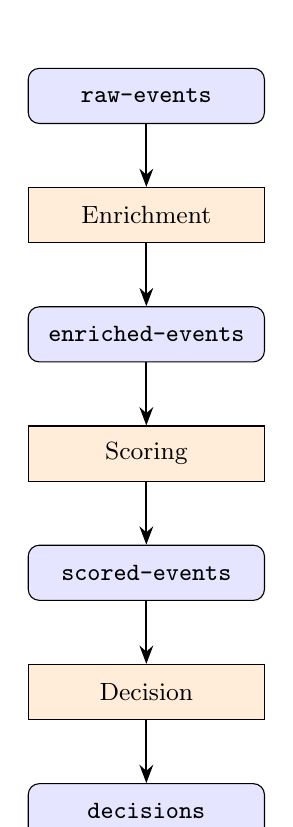
\begin{tikzpicture}[
    node distance=0.8cm,
    topic/.style={draw, rounded corners, fill=blue!10, minimum width=3cm,
                  minimum height=0.7cm, font=\small\ttfamily, align=center},
    service/.style={draw, fill=orange!15, minimum width=3cm,
                    minimum height=0.7cm, font=\small, align=center},
    arrow/.style={-{Stealth}, thick}
]
\node[topic]   (raw)      {raw-events};
\node[service, below=of raw]      (enr)      {Enrichment};
\node[topic,   below=of enr]      (enriched) {enriched-events};
\node[service, below=of enriched] (scr)      {Scoring};
\node[topic,   below=of scr]      (scored)   {scored-events};
\node[service, below=of scored]   (dec)      {Decision};
\node[topic,   below=of dec]      (decisions){decisions};

\draw[arrow] (raw)      -- (enr);
\draw[arrow] (enr)      -- (enriched);
\draw[arrow] (enriched) -- (scr);
\draw[arrow] (scr)      -- (scored);
\draw[arrow] (scored)   -- (dec);
\draw[arrow] (dec)      -- (decisions);
\end{tikzpicture}
\caption{Streaming topic chain}
\label{fig:topic-chain}
\end{figure}

All four topics share a single partition key: \texttt{client\_id}. This is a
deliberate constraint. The LSTM model treats each client's transaction history
as a temporal sequence across all four operation types. If operations were split
across separate topics (one per operation type), cross-operation ordering would
be lost --- a retrait followed by a versement five minutes later would arrive on
different topics with no guaranteed relative ordering. A single topic partitioned
by \texttt{client\_id} guarantees that all events for a given client arrive at
the Enrichment Service in the order they occurred, preserving the temporal
signal the LSTM depends on.

\subsection{Broker Choice: RedPanda}

RedPanda provides a Kafka-compatible API without the JVM or ZooKeeper
dependency. This matters in a Docker Compose deployment where every service
competes for memory. A Kafka cluster requires a minimum of three containers
(ZooKeeper + broker + schema registry), while RedPanda runs as a single
container with the same producer/consumer API. The streaming wrappers use
\texttt{kafka-python} and are unaware they are communicating with RedPanda
rather than Kafka --- the switch is transparent at the application level.

\subsection{Consumer Groups and Offset Management}

Each service registers a dedicated consumer group
(\texttt{enrichment-service}, \texttt{scoring-service},
\texttt{decision-service}). Consumer groups provide two guarantees that the
pipeline relies on. First, offset tracking: if a service restarts, it resumes
from the last committed offset rather than replaying the entire topic. Second,
horizontal scalability: adding a second instance of the Enrichment Service
automatically splits partitions across the two consumers, doubling throughput
without code changes. In the current deployment, each service runs as a single
consumer, but the architecture supports scaling out by adding replicas.

% ═══════════════════════════════════════════════════════════
\section{Core Extraction Pattern}
% ═══════════════════════════════════════════════════════════

The system supports three execution paths that all require the same computation:

\begin{enumerate}
    \item \textbf{Streaming} --- Kafka consumer loop, one event at a time,
          writes to Redis buffers
    \item \textbf{Batch} --- Airflow DAG iterating over PostgreSQL rows,
          no Redis interaction
    \item \textbf{Simulation API} --- FastAPI endpoint, synchronous
          request-response, read-only Redis access
\end{enumerate}

Duplicating the enrichment, scoring, or decision logic across these three paths
would create a maintenance burden and a drift risk: any feature computation
change would need to be applied in three places. The solution is a consistent
separation between \emph{core logic} and \emph{transport wrappers}.

\subsection{Core Modules}

Each pipeline stage has a core module that encapsulates all domain logic:

\begin{table}[H]
\centering
\caption{Core modules and their responsibilities}
\label{tab:core-modules}
\begin{tabular}{@{}lll@{}}
\toprule
\textbf{Core} & \textbf{File} & \textbf{Public Method} \\
\midrule
EnrichmentCore & \texttt{src/enrichment/core.py} & \texttt{enrich\_event()} \\
ScoringCore    & \texttt{src/scoring/core.py}     & \texttt{score\_event()} \\
DecisionCore   & \texttt{src/decision/core.py}    & \texttt{decide\_event()} \\
\bottomrule
\end{tabular}
\end{table}

Each core receives its dependencies via constructor injection: a Redis client,
model objects, or configuration. The core exposes a single public method
(fa\c{c}ade pattern) and uses private helpers for sub-steps. Critically, the
cores have no knowledge of Kafka, Airflow, or FastAPI --- they operate on
Python dictionaries and return Python dictionaries.

\subsection{Thin Streaming Wrappers}

The Kafka-specific logic lives in \texttt{src/streaming/}, where each wrapper
file does exactly three things: poll a topic, call the core's public method,
and produce the result to the next topic. The wrapper receives its core
instance via dependency injection at startup. The \texttt{\_\_main\_\_} block
is the sole wiring point: it creates the Redis client, loads models, constructs
the core, injects it into the wrapper, and starts the poll loop.

This separation has a concrete payoff. When the batch pipeline was rewritten
(Section~\ref{sec:batch-integration}), it imported \texttt{EnrichmentCore}
and called the same \texttt{\_compute\_features()} method. When the simulation
API was built, it imported all three cores and wired them with a shared Redis
client. In both cases, zero feature computation code was duplicated.

% ═══════════════════════════════════════════════════════════
\section{Dead Letter Queue and Fault Tolerance}
\label{sec:dlq}
% ═══════════════════════════════════════════════════════════

In a streaming pipeline, a single malformed event can block an entire consumer
if the error is not handled. The fault tolerance layer classifies failures into
two categories and applies different strategies to each.

\subsection{Failure Classification}

\paragraph{Poison pills} (\texttt{KeyError}, \texttt{ValueError},
\texttt{JSONDecodeError}) are structurally invalid events that will never
succeed regardless of how many times they are retried. These are routed to
the DLQ immediately with \texttt{retry\_count=0}.

\paragraph{Transient failures} (\texttt{redis.ConnectionError},
\texttt{psycopg2.OperationalError}, network timeouts) are infrastructure
errors that may resolve on their own. The consumer applies exponential
backoff (1s, 2s, 4s) and retries up to 3 times. If all retries fail, the
event is routed to the DLQ with \texttt{retry\_count=3}.

The distinction matters because the two classes require opposite responses.
Retrying a poison pill wastes time and will never succeed. Immediately
discarding a transient failure loses an event that would have succeeded one
second later when Redis reconnected.

\subsection{ResilientConsumer}

The \texttt{ResilientConsumer} class (\texttt{src/streaming/dlq.py}) wraps all
three streaming services. It intercepts exceptions from the core's public
method, classifies them using an \texttt{isinstance} check against a
\texttt{TRANSIENT\_ERRORS} tuple, applies the appropriate strategy, and
produces failed events to a single \texttt{dlq} topic.

Each DLQ message is wrapped in a metadata envelope:

\begin{table}[H]
\centering
\caption{DLQ envelope fields}
\label{tab:dlq-envelope}
\begin{tabular}{@{}lp{7.5cm}@{}}
\toprule
\textbf{Field} & \textbf{Description} \\
\midrule
\texttt{original\_event}  & The raw event that caused the failure \\
\texttt{source\_topic}    & Topic the event was consumed from \\
\texttt{service}          & Service that failed (enrichment, scoring, decision) \\
\texttt{error\_type}      & Exception class name \\
\texttt{error\_message}   & Exception message string \\
\texttt{stacktrace}       & Full Python traceback \\
\texttt{retry\_count}     & Number of retries attempted before routing to DLQ \\
\texttt{max\_retries}     & Configured maximum (3 for transient errors) \\
\texttt{timestamps}       & First failure and last failure timestamps \\
\bottomrule
\end{tabular}
\end{table}

The envelope preserves enough context for an operator to diagnose the failure,
replay the event after fixing the root cause, and distinguish between
infrastructure outages (transient, clustered in time) and data quality issues
(poison pills, scattered across clients).

\subsection{Structured Logging}

The streaming services use structured JSON logging rather than plain
\texttt{print()} statements. A \texttt{JsonFormatter} class
(\texttt{src/streaming/logger.py}) formats every log line as a JSON object
with a fixed schema: \texttt{timestamp} (UTC ISO 8601), \texttt{service},
\texttt{level}, \texttt{message}, and optional contextual fields
(\texttt{event\_id}, \texttt{client\_id}, \texttt{error\_type},
\texttt{retry\_count}, \texttt{score}, \texttt{alert\_tier}).

A \texttt{setup\_logger(service\_name)} factory function creates a named
logger with the JSON formatter attached. Each streaming service calls
this factory once at startup. The structured format enables log aggregation
tools to filter, group, and alert on specific fields without parsing free-text
messages --- for example, filtering all log lines where
\texttt{error\_type = "redis.ConnectionError"} to detect infrastructure
degradation.

% ═══════════════════════════════════════════════════════════
\section{Enrichment Service}
% ═══════════════════════════════════════════════════════════

The Enrichment Service consumes raw events, computes 30 contrast features by
comparing the current event against the client's historical profile, and
produces enriched events for the Scoring Service.

\subsection{Data Sources}

For each incoming event, the service fetches two categories of data from Redis:

\begin{table}[H]
\centering
\caption{Enrichment Service data sources}
\label{tab:enrichment-sources}
\begin{tabular}{@{}llp{6cm}@{}}
\toprule
\textbf{Source} & \textbf{Redis Key} & \textbf{Content} \\
\midrule
Client profile & \texttt{profile:client:\{id\}} & Batch-computed statistics:
    amount means/stds per operation, operation mix distributions, archetype,
    account age \\
Client buffer  & \texttt{buffer:client:\{id\}} & Last 50 raw event summaries
    (timestamp, amount, operation, payload) for velocity features \\
Employee buffer & \texttt{buffer:employee:\{id\}} & Recent events processed
    by this employee for peer comparison features \\
\bottomrule
\end{tabular}
\end{table}

The client profile is rebuilt nightly by the batch pipeline
(Section~\ref{sec:batch-integration}). The buffers are updated per-event by
the Enrichment Service itself after feature computation.

\subsection{Feature Computation}

The 30 enriched features are organized into categories that reflect how each
feature is derived:

\begin{table}[H]
\centering
\caption{Enriched feature categories}
\label{tab:enriched-features-ch5}
\begin{tabular}{@{}lrl@{}}
\toprule
\textbf{Category} & \textbf{Count} & \textbf{Source} \\
\midrule
Raw event (amount, hour, operation one-hot, branch match) & 7 & Event \\
Amount contrast (z-score, ratio to mean, threshold flags) & 6 & Event + Profile \\
Operation contrast (deviation from expected mix)          & 1 & Event + Profile \\
Timing contrast (hour deviation, day-of-month deviation)  & 2 & Event + Profile \\
Counterparty contrast (known vs. new)                     & 1 & Event payload \\
Velocity (24h/7d counts, cumulative amount, duplicates)   & 5 & Redis buffer \\
Employee (transaction count, client pair count)            & 2 & Redis buffer \\
Context (archetype one-hot, account age)                  & 6 & Profile \\
\bottomrule
\end{tabular}
\end{table}

The term \emph{contrast feature} is central to the design. Raw event fields
(amount, hour, operation type) carry no anomaly signal on their own --- a
10{,}000~DT versement is normal for a big business client but extreme for a
student. Every feature is computed relative to the client's own baseline,
transforming absolute values into deviations that are comparable across
archetypes.

\subsection{Amount Statistics Fallback Chain}

When a client has no 30-day transaction history for a given operation type
(common for infrequent operations like cheque deposits), the amount z-score
computation would fail with a division-by-zero. The service applies a three-level
fallback chain: 30-day statistics first, then 90-day statistics, then the
archetype baseline. This ensures every event receives a meaningful contrast
score regardless of the client's transaction density.

\subsection{Sequence Buffer Management}

After computing the 30 features, the Enrichment Service appends the
\emph{unscaled} feature vector to \texttt{sequence:client:\{id\}} in Redis,
capped at 10 entries. The Scoring Service later retrieves this sequence,
scales it using the training-time \texttt{StandardScaler}, and feeds it to
the LSTM. The features are stored unscaled because the scaler is owned by
the Scoring Service --- storing pre-scaled features would create a coupling
between the Enrichment Service and the scaler version, breaking independence
during model retraining.

% ═══════════════════════════════════════════════════════════
\section{Scoring Service}
% ═══════════════════════════════════════════════════════════

The Scoring Service consumes enriched events, runs both anomaly detection
models, and produces a fused anomaly score with optional SHAP explanations.

\subsection{Score Fusion}

The system runs two complementary models on every event:

\begin{itemize}
    \item \textbf{Autoencoder} --- computes a reconstruction error that
          measures how different the current event is from the ``normal''
          patterns learned during training. The error is converted to a
          percentile rank against the training distribution.
    \item \textbf{LSTM} --- evaluates how surprising the current event is
          given the client's recent sequence of transactions. The prediction
          error is similarly converted to a percentile rank.
\end{itemize}

The two scores are combined using a sigmoid-weighted fusion controlled by
account maturity:

\[
w_{\text{lstm}} = \sigma\!\left(\frac{d - 90}{15}\right)
\]

where $d$ is the number of days since the account was opened, and $\sigma$ is
the logistic function. For accounts younger than ${\sim}75$ days, the
Autoencoder dominates ($w_{\text{lstm}} \approx 0$). For mature accounts
($d > 105$), the LSTM dominates ($w_{\text{lstm}} \approx 1$). The midpoint
of 90 days reflects the minimum history needed for the LSTM's sequence model
to produce reliable predictions.

\[
\text{fused\_score} = (1 - w_{\text{lstm}}) \cdot s_{\text{ae}}
                    + w_{\text{lstm}} \cdot s_{\text{lstm}}
\]

\subsection{Cold-Start Guard}

Clients with fewer than 5 events in their sequence buffer present a distinct
problem. Their velocity features (\texttt{tx\_count\_24h},
\texttt{cumulative\_amount\_24h}) sit far outside the training distribution,
which applied a 21-day warm-up filter. Without a guard, these zero-velocity
vectors produce AE reconstruction errors that map to percentiles above 0.99,
generating false BLOCK-tier alerts for every new client.

The Scoring Service detects cold-start conditions by checking the sequence
buffer length in Redis. When the buffer contains fewer than 5 events, it
returns a neutral score of 0.5 with $w_{\text{lstm}} = 0$ and no SHAP
explanations. This creates a three-tier progression:

\begin{table}[H]
\centering
\caption{Scoring behavior by buffer maturity}
\label{tab:cold-start-ch5}
\begin{tabular}{@{}rll@{}}
\toprule
\textbf{Buffer Size} & \textbf{Scoring Mode} & \textbf{Rationale} \\
\midrule
0--4 events  & Neutral (0.5)    & Insufficient data for meaningful scoring \\
5--9 events  & AE only          & Enough for point anomaly, not for sequence \\
10+ events   & Full AE + LSTM   & Both models have sufficient context \\
\bottomrule
\end{tabular}
\end{table}

\subsection{Conditional SHAP}

SHAP explanations are computationally expensive --- KernelExplainer for the
Autoencoder requires multiple model evaluations per event. To avoid wasting
computation on events that will be classified as INFO, the Scoring Service
only generates SHAP explanations when the fused score exceeds the first
threshold ($T_1 = 0.95$). Events below this threshold are overwhelmingly
normal; explanations for them would never reach the supervisor's screen.

% ═══════════════════════════════════════════════════════════
\section{Decision Service}
% ═══════════════════════════════════════════════════════════

The Decision Service consumes scored events and produces the final alert
decision: an alert tier (INFO, REVIEW, ALERT, or BLOCK) with an explanation
combining model scores and regulatory rule triggers.

\subsection{Alert Tier Assignment}

The base tier is derived from the fused anomaly score using three thresholds:

\begin{table}[H]
\centering
\caption{Score-to-tier mapping}
\label{tab:tier-thresholds}
\begin{tabular}{@{}lll@{}}
\toprule
\textbf{Score Range} & \textbf{Tier} & \textbf{Supervisor Action} \\
\midrule
$< 0.95$ (T\textsubscript{1})                          & INFO   & No action required \\
$\geq 0.95$ and $< 0.99$ (T\textsubscript{2})          & REVIEW & Manual review recommended \\
$\geq 0.99$ and $< 0.999$ (T\textsubscript{3})         & ALERT  & Immediate review required \\
$\geq 0.999$                                            & BLOCK  & Transaction held pending review \\
\bottomrule
\end{tabular}
\end{table}

\subsection{Regulatory Rules}

After the score-based tier is assigned, 8 regulatory rules are evaluated. Each
rule can \emph{escalate} the tier but never \emph{de-escalate} it. This is a
deliberate design constraint: if the model assigns ALERT and a rule would
suggest REVIEW, the tier stays at ALERT. Regulatory flags are always logged
for audit purposes regardless of whether they change the tier.

The escalation-only principle exists because rules encode hard regulatory
requirements (BCT reporting thresholds, LAB/FT structuring patterns) that
must never be overridden by a statistical model. A model might assign a low
score to a transaction that happens to hit a regulatory threshold; the rule
ensures the supervisor still sees it.

Selected rules illustrate the pattern:

\begin{itemize}
    \item \textbf{BCT threshold rule} --- any single transaction exceeding
          10{,}000~DT escalates to at least REVIEW, but only when the amount
          z-score $\geq 2$. The z-score guard prevents routine big-business
          transactions (where 10{,}000~DT is normal) from flooding the
          REVIEW queue.
    \item \textbf{Smurfing detection} --- multiple versements in the
          8{,}000--9{,}999~DT band within 48 hours escalates to ALERT,
          targeting deliberate structuring below the reporting threshold.
    \item \textbf{Cheque cap rule} --- any cheque exceeding 30{,}000~DT
          (the cap established by Law n\textsuperscript{o}41-2024, effective
          February 2025) escalates to BLOCK.
\end{itemize}

\subsection{Cold-Start Tier Cap}

Events flagged as \texttt{cold\_start=True} by the Scoring Service still pass
through all regulatory rules --- a genuinely suspicious transaction from a new
client must still trigger the appropriate flags. However, the Decision Service
caps the final tier at REVIEW for cold-start events. This prevents the neutral
score of 0.5 from being escalated to ALERT or BLOCK by rules alone, which would
generate high-priority alerts for clients who simply have not built enough
history yet. The cap is logged in the decision reasons so supervisors understand
why the tier is limited.

% ═══════════════════════════════════════════════════════════
\section{Sink Consumers}
\label{sec:sinks}
% ═══════════════════════════════════════════════════════════

Two sink consumers persist streaming data to PostgreSQL for historical
querying, dashboard display, and the retraining feedback loop.

\subsection{Raw Events Sink}

The \texttt{raw\_events\_sink} consumes from the \texttt{raw-events} topic
and inserts each event into the \texttt{transactions} table. This provides the
permanent record that the batch pipeline uses for nightly profile rebuilds
and that the dashboard uses for transaction history display.

\subsection{Decisions Sink}

The \texttt{decisions\_sink} consumes from the \texttt{decisions} topic and
performs two writes per event:

\begin{enumerate}
    \item \textbf{PostgreSQL} --- inserts into the \texttt{alerts} table with
          the alert tier, fused score, SHAP explanation (stored as JSONB), and
          all triggered rule names. The \texttt{supervisor\_decision} and
          \texttt{decision\_timestamp} fields are initially \texttt{NULL},
          populated later when the supervisor confirms or rejects the alert
          through the dashboard.
    \item \textbf{Redis} --- increments risk history counters for the client
          (\texttt{risk:client:\{id\}}), tracking the count of alerts per tier
          over rolling windows. These counters feed back into the enrichment
          features for subsequent events.
\end{enumerate}

\subsection{Deliberate FK Omission}

The \texttt{alerts} table does not have a foreign key constraint to the
\texttt{transactions} table, despite both containing the same
\texttt{event\_id}. This is intentional. The two sink consumers run in
parallel: one consumes \texttt{raw-events}, the other consumes
\texttt{decisions}. Because the decision pipeline adds latency (enrichment,
scoring, rule evaluation), the decisions sink may attempt to insert an alert
before the raw events sink has inserted the corresponding transaction. A
foreign key constraint would cause intermittent insertion failures depending
on which consumer is faster at any given moment. The \texttt{event\_id} field
still links the two tables logically; the constraint is enforced at the
application level rather than the database level.


% ═══════════════════════════════════════════════════════════
\section{Data Persistence Layer}
\label{sec:persistence}
% ═══════════════════════════════════════════════════════════

The PostgreSQL database serves as the cold store for the entire system. It
receives writes from two streaming sinks and the batch pipeline, and provides
reads for the dashboard, the batch profile rebuild, and the retraining
pipeline. Figure~\ref{fig:er-diagram} shows the table relationships.

\begin{figure}[H]
\centering
\resizebox{\textwidth}{!}{%
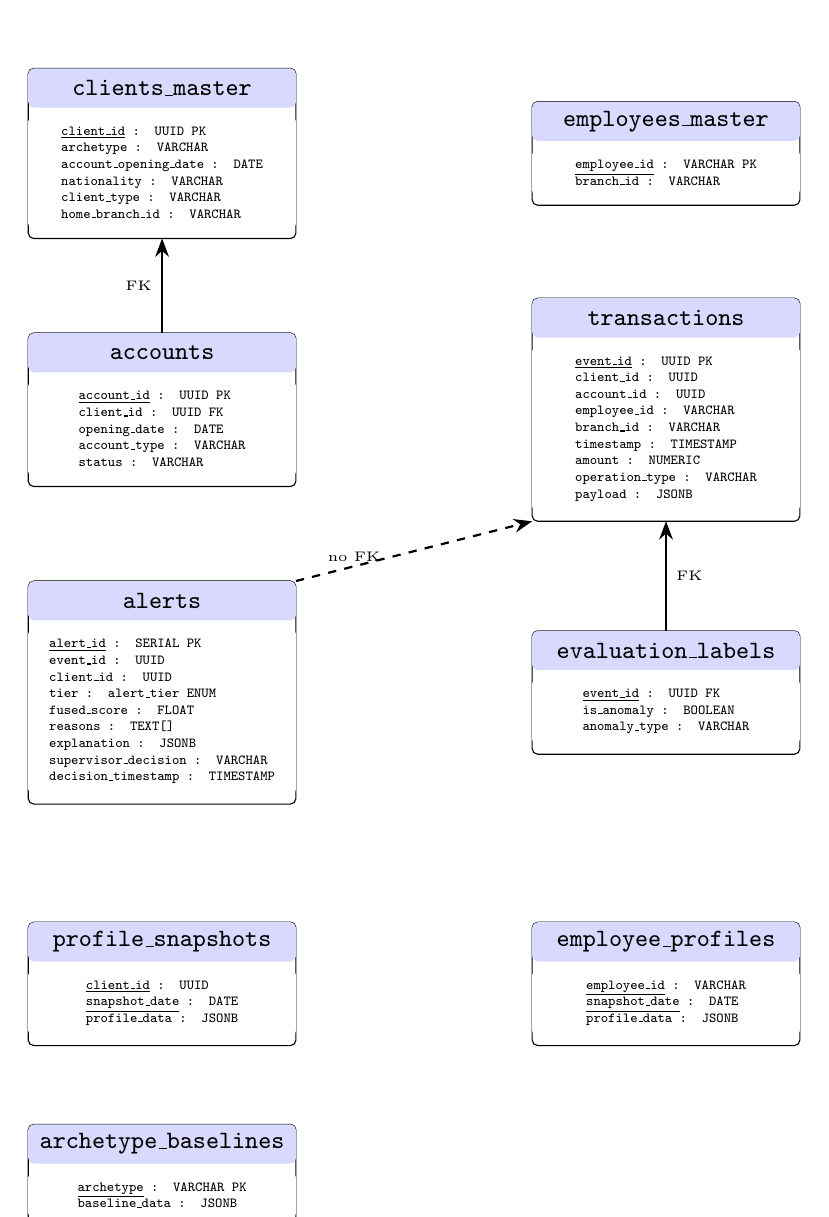
\begin{tikzpicture}[
    node distance=1.2cm and 1.8cm,
    every node/.style={font=\small},
    table/.style={
        draw, rectangle, rounded corners=2pt,
        inner sep=0pt, outer sep=0pt,
        minimum width=3.4cm
    },
    header/.style={
        fill=blue!15, font=\small\bfseries\ttfamily,
        minimum width=3.4cm, minimum height=0.5cm, align=center
    },
    cols/.style={
        fill=white, font=\tiny\ttfamily,
        minimum width=3.4cm, align=left, inner sep=4pt
    },
    fk/.style={-{Stealth}, thick},
    nofk/.style={-{Stealth}, thick, dashed},
]

% ── clients_master ──
\node[table] (clients) {
    \begin{tabular}{@{}c@{}}
    \tikz\node[header]{clients\_master};\\[-0.4pt]
    \tikz\node[cols]{%
        \underline{client\_id} : UUID PK\\
        archetype : VARCHAR\\
        account\_opening\_date : DATE\\
        nationality : VARCHAR\\
        client\_type : VARCHAR\\
        home\_branch\_id : VARCHAR
    };
    \end{tabular}
};

% ── employees_master ──
\node[table, right=3cm of clients] (employees) {
    \begin{tabular}{@{}c@{}}
    \tikz\node[header]{employees\_master};\\[-0.4pt]
    \tikz\node[cols]{%
        \underline{employee\_id} : VARCHAR PK\\
        branch\_id : VARCHAR
    };
    \end{tabular}
};

% ── accounts ──
\node[table, below=of clients] (accounts) {
    \begin{tabular}{@{}c@{}}
    \tikz\node[header]{accounts};\\[-0.4pt]
    \tikz\node[cols]{%
        \underline{account\_id} : UUID PK\\
        client\_id : UUID FK\\
        opening\_date : DATE\\
        account\_type : VARCHAR\\
        status : VARCHAR
    };
    \end{tabular}
};

% ── transactions ──
\node[table, right=3cm of accounts] (transactions) {
    \begin{tabular}{@{}c@{}}
    \tikz\node[header]{transactions};\\[-0.4pt]
    \tikz\node[cols]{%
        \underline{event\_id} : UUID PK\\
        client\_id : UUID\\
        account\_id : UUID\\
        employee\_id : VARCHAR\\
        branch\_id : VARCHAR\\
        timestamp : TIMESTAMP\\
        amount : NUMERIC\\
        operation\_type : VARCHAR\\
        payload : JSONB
    };
    \end{tabular}
};

% ── alerts ──
\node[table, below=of accounts] (alerts) {
    \begin{tabular}{@{}c@{}}
    \tikz\node[header]{alerts};\\[-0.4pt]
    \tikz\node[cols]{%
        \underline{alert\_id} : SERIAL PK\\
        event\_id : UUID\\
        client\_id : UUID\\
        tier : alert\_tier ENUM\\
        fused\_score : FLOAT\\
        reasons : TEXT[]\\
        explanation : JSONB\\
        supervisor\_decision : VARCHAR\\
        decision\_timestamp : TIMESTAMP
    };
    \end{tabular}
};

% ── evaluation_labels ──
\node[table, right=3cm of alerts] (eval) {
    \begin{tabular}{@{}c@{}}
    \tikz\node[header]{evaluation\_labels};\\[-0.4pt]
    \tikz\node[cols]{%
        \underline{event\_id} : UUID FK\\
        is\_anomaly : BOOLEAN\\
        anomaly\_type : VARCHAR
    };
    \end{tabular}
};

% ── profile_snapshots ──
\node[table, below=1.5cm of alerts] (profiles) {
    \begin{tabular}{@{}c@{}}
    \tikz\node[header]{profile\_snapshots};\\[-0.4pt]
    \tikz\node[cols]{%
        \underline{client\_id} : UUID\\
        \underline{snapshot\_date} : DATE\\
        profile\_data : JSONB
    };
    \end{tabular}
};

% ── employee_profile_snapshots ──
\node[table, right=3cm of profiles] (emp_profiles) {
    \begin{tabular}{@{}c@{}}
    \tikz\node[header]{employee\_profiles};\\[-0.4pt]
    \tikz\node[cols]{%
        \underline{employee\_id} : VARCHAR\\
        \underline{snapshot\_date} : DATE\\
        profile\_data : JSONB
    };
    \end{tabular}
};

% ── archetype_baselines ──
\node[table, below=1cm of profiles] (baselines) {
    \begin{tabular}{@{}c@{}}
    \tikz\node[header]{archetype\_baselines};\\[-0.4pt]
    \tikz\node[cols]{%
        \underline{archetype} : VARCHAR PK\\
        baseline\_data : JSONB
    };
    \end{tabular}
};

% ── Relationships ──
\draw[fk] (accounts.north) -- node[left, font=\tiny, pos=0.5] {FK} (clients.south);
\draw[fk] (eval.north) -- node[right, font=\tiny, pos=0.5] {FK} (transactions.south);
\draw[nofk] (alerts.north east) -- node[left, font=\tiny, pos=0.4] {no FK} (transactions.south west);

\end{tikzpicture}
}%
\caption{Database schema --- entity relationship diagram. Solid arrows represent
         foreign key constraints; the dashed arrow between \texttt{alerts} and
         \texttt{transactions} indicates a logical link without a database-level
         constraint (Section~\ref{sec:sinks}).}
\label{fig:er-diagram}
\end{figure}

\subsection{Master Tables}

Two master tables store the static reference data loaded once from the
generator output:

\begin{table}[H]
\centering
\caption{\texttt{clients\_master} --- one row per client}
\label{tab:clients-master}
\begin{tabularx}{\textwidth}{@{}llX@{}}
\toprule
\textbf{Column} & \textbf{Type} & \textbf{Description} \\
\midrule
\texttt{client\_id}           & UUID PK      & Unique client identifier \\
\texttt{archetype}            & VARCHAR(20)  & One of: salaried, small\_business, student, retiree, big\_business \\
\texttt{account\_opening\_date} & DATE        & Used to compute \texttt{account\_age\_days} during enrichment \\
\texttt{nationality}          & VARCHAR(5)   & Default \texttt{TN} (Tunisia) \\
\texttt{client\_type}         & VARCHAR(30)  & Regulatory classification: personne\_physique or personne\_morale \\
\texttt{home\_branch\_id}     & VARCHAR(10)  & Primary branch for branch-match feature \\
\bottomrule
\end{tabularx}
\end{table}

\begin{table}[H]
\centering
\caption{\texttt{employees\_master} --- one row per teller}
\label{tab:employees-master}
\begin{tabularx}{\textwidth}{@{}llX@{}}
\toprule
\textbf{Column} & \textbf{Type} & \textbf{Description} \\
\midrule
\texttt{employee\_id} & VARCHAR(10) PK & Teller identifier (e.g., \texttt{EMP-0001}) \\
\texttt{branch\_id}   & VARCHAR(10)    & Assigned branch (exactly 2 employees per branch) \\
\bottomrule
\end{tabularx}
\end{table}

\subsection{Transaction and Event Tables}

\begin{table}[H]
\centering
\caption{\texttt{transactions} --- populated by the raw events sink}
\label{tab:transactions-table}
\begin{tabularx}{\textwidth}{@{}llX@{}}
\toprule
\textbf{Column} & \textbf{Type} & \textbf{Description} \\
\midrule
\texttt{event\_id}       & UUID PK      & Unique event identifier \\
\texttt{client\_id}      & UUID         & Client performing the operation \\
\texttt{account\_id}     & UUID         & Target account \\
\texttt{employee\_id}    & VARCHAR(10)  & Teller processing the operation \\
\texttt{branch\_id}      & VARCHAR(10)  & Branch where the operation occurred \\
\texttt{timestamp}       & TIMESTAMP    & Operation timestamp \\
\texttt{amount}          & NUMERIC      & Transaction amount in TND \\
\texttt{currency}        & VARCHAR(3)   & Always \texttt{TND} \\
\texttt{channel}         & VARCHAR(20)  & Always \texttt{guichet} (teller window) \\
\texttt{operation\_type} & VARCHAR(20)  & One of: retrait, versement, virement, cheque \\
\texttt{payload}         & JSONB        & Operation-specific fields (beneficiary, cheque number, etc.) \\
\bottomrule
\end{tabularx}
\end{table}

\begin{table}[H]
\centering
\caption{\texttt{evaluation\_labels} --- ground truth for model evaluation}
\label{tab:eval-labels}
\begin{tabularx}{\textwidth}{@{}llX@{}}
\toprule
\textbf{Column} & \textbf{Type} & \textbf{Description} \\
\midrule
\texttt{event\_id}     & UUID FK $\rightarrow$ \texttt{transactions} & Links to the original event \\
\texttt{is\_anomaly}   & BOOLEAN  & Generator oracle label \\
\texttt{anomaly\_type} & VARCHAR  & Scenario name (e.g., smurfing, amount\_spike) or \texttt{NULL} \\
\bottomrule
\end{tabularx}
\end{table}

The \texttt{evaluation\_labels} table is separated from \texttt{transactions}
by design. Oracle labels are generator metadata used exclusively for model
evaluation --- they do not exist in a production system with real data. Keeping
them in a separate table makes it trivial to exclude them from production
deployments without modifying the transaction schema.

\subsection{Alerts Table}

\begin{table}[H]
\centering
\caption{\texttt{alerts} --- populated by the decisions sink}
\label{tab:alerts-table}
\begin{tabularx}{\textwidth}{@{}llX@{}}
\toprule
\textbf{Column} & \textbf{Type} & \textbf{Description} \\
\midrule
\texttt{alert\_id}            & SERIAL PK    & Auto-incrementing alert identifier \\
\texttt{event\_id}            & UUID         & References the triggering event (no FK --- see Section~\ref{sec:sinks}) \\
\texttt{client\_id}           & UUID         & Client involved \\
\texttt{employee\_id}         & VARCHAR(10)  & Teller who processed the operation \\
\texttt{branch\_id}           & VARCHAR(10)  & Branch location \\
\texttt{timestamp}            & TIMESTAMP    & Event timestamp \\
\texttt{amount}               & NUMERIC      & Transaction amount \\
\texttt{operation\_type}      & VARCHAR(20)  & Operation type \\
\texttt{tier}                 & alert\_tier ENUM & INFO, REVIEW, ALERT, or BLOCK \\
\texttt{fused\_score}         & FLOAT        & Combined AE + LSTM anomaly score \\
\texttt{reasons}              & TEXT[]       & Array of triggered rule names and score-based reasons \\
\texttt{regulatory\_flags}    & TEXT[]       & Regulatory rules that fired (logged regardless of tier impact) \\
\texttt{explanation}          & JSONB        & SHAP explanation with \texttt{reasons} (NLG text) and \texttt{raw} (feature-level detail) \\
\texttt{supervisor\_decision} & VARCHAR(10)  & \texttt{pending}, \texttt{confirmed}, or \texttt{rejected} \\
\texttt{supervisor\_notes}    & TEXT         & Free-text supervisor commentary \\
\texttt{decision\_timestamp}  & TIMESTAMP    & When the supervisor acted \\
\bottomrule
\end{tabularx}
\end{table}

The \texttt{tier} column uses a PostgreSQL ENUM type rather than a VARCHAR.
This enforces valid values at the database level and enables direct ordering
(\texttt{INFO < REVIEW < ALERT < BLOCK}) in queries without a CASE expression.

\subsection{Profile and Baseline Tables}

Three tables support the batch profile rebuild pipeline:

\begin{table}[H]
\centering
\caption{Profile and baseline tables}
\label{tab:profile-tables}
\begin{tabularx}{\textwidth}{@{}llX@{}}
\toprule
\textbf{Table} & \textbf{Key} & \textbf{Content} \\
\midrule
\texttt{profile\_snapshots}          & (\texttt{client\_id}, \texttt{snapshot\_date})
    & Client profile as JSONB: transaction statistics, behavioral distributions,
      financial state, risk history, recent events buffer \\
\addlinespace
\texttt{employee\_profile\_snapshots} & (\texttt{employee\_id}, \texttt{snapshot\_date})
    & Employee profile as JSONB: processed transaction stats, client distribution,
      peer comparison z-scores \\
\addlinespace
\texttt{archetype\_baselines}        & \texttt{archetype} PK
    & Per-archetype reference statistics as JSONB: mean amounts, operation mix,
      frequency norms. Used as the final fallback in the amount statistics
      fallback chain \\
\bottomrule
\end{tabularx}
\end{table}

Profiles are stored as JSONB rather than as individual columns. A client
profile contains approximately 194 fields across 6 categories; normalizing
these into columns would produce an unwieldy table that changes shape every
time a feature is added. JSONB stores the profile as a single document,
and the nightly rebuild overwrites it atomically via \texttt{ON CONFLICT}
upsert. The tradeoff is that individual fields cannot be indexed or queried
efficiently, but the access pattern (load entire profile into Redis) does not
require per-field queries.

% ═══════════════════════════════════════════════════════════
\section{Batch Integration}
\label{sec:batch-integration}
% ═══════════════════════════════════════════════════════════

The streaming pipeline depends on client profiles that are too expensive to
recompute on every event. A nightly batch pipeline rebuilds these profiles
from the full transaction history in PostgreSQL and loads the results into
Redis for the next day's streaming consumption.

\subsection{Nightly Profile Rebuild}

An Airflow DAG (\texttt{nightly\_profiles}) runs eight tasks with validation
gates between stages:

\begin{enumerate}
    \item Rebuild client profile snapshots from the \texttt{transactions} table
    \item Validate snapshot completeness (row counts, null checks)
    \item Rebuild employee profile snapshots
    \item Validate employee snapshots
    \item Recompute archetype baselines
    \item Validate baselines
    \item Hydrate Redis with updated profiles
    \item Run a smoke test (score a sample event with the new profiles)
\end{enumerate}

Each task uses \texttt{ON CONFLICT} upserts on its target table, making every
task individually retriable. If an Airflow task fails mid-execution and is
retried, the upsert ensures that partially-written rows are overwritten
rather than duplicated.

\subsection{Feature Parity Guarantee}

The batch profile computation calls the same
\texttt{EnrichmentCore.\_compute\_features()} method used by the streaming
pipeline. The method is a pure function: it takes an event, a profile, and
buffer data as arguments and returns 30 features with no side effects. The
batch script passes the archetype baseline as a parameter rather than
fetching it from Redis, which is the only difference from the streaming path.

This design guarantees that the features used to rebuild profiles overnight are
computed with identical logic to the features produced in real time. Any change
to the feature computation --- adding a feature, modifying a z-score formula,
adjusting the fallback chain --- is automatically reflected in both paths
because both paths call the same function.

\subsection{Streaming--Batch Coordination}

The current deployment does not pause streaming consumers during the batch
rebuild window. In practice, the nightly DAG runs during low-traffic hours
when transaction volume is minimal, and the Redis hydration step atomically
overwrites profile keys. A brief window exists where a streaming event could
read a stale profile (pre-rebuild) and then the next event reads the updated
profile, creating a one-event inconsistency. For the current deployment this
is acceptable; a production system would implement a coordination mechanism
such as pausing consumers during the hydration step or using Redis
transactions to swap profile versions atomically. This is documented as
future work in Chapter~\ref{ch:roadmap}.

% --- Chapter 6 ---
\chapter{MLOps, Observability, and Production Readiness}
\label{ch:mlops}
This chapter covers the infrastructure that surrounds the machine learning
models: how experiments are tracked, how models are promoted to production,
how the system detects when retraining is needed, and how operational health
is monitored. Together, these components close the loop between model serving
and model improvement.

% ═══════════════════════════════════════════════════════════
\section{MLOps Lifecycle Overview}
\label{sec:mlops-lifecycle}
% ═══════════════════════════════════════════════════════════

A trained model that cannot be retrained, versioned, or monitored is a
liability rather than an asset. The MLOps layer transforms the models
described in Chapter~\ref{ch:training} from static artifacts into a managed
lifecycle with four stages:

\begin{enumerate}
    \item \textbf{Train} --- execute a training job that produces a candidate
          model with logged hyperparameters and metrics.
    \item \textbf{Promote} --- compare the candidate against the current
          production model and replace it only if performance is equal or
          better.
    \item \textbf{Serve} --- the streaming pipeline loads the promoted model
          from a shared volume mount, requiring no image rebuild.
    \item \textbf{Monitor} --- observe the score distribution in production
          and trigger a new training cycle when drift is detected or
          supervisor feedback indicates degradation.
\end{enumerate}

The lifecycle is largely automated. Training, promotion, serving, and
monitoring all run without human intervention. The single human touch point
is the supervisor confirming or rejecting alerts in the dashboard
(Section~\ref{sec:feedback-loop}), which feeds one of the three retraining
triggers. The promotion gate in particular has no manual approval step
between a candidate model and production deployment --- a deliberate scope
decision discussed in Section~\ref{sec:promotion-gate}.

Three independent triggers can initiate a new training cycle: a weekly
schedule, a drift alert from the monitoring stack, and a supervisor feedback
divergence signal. Sections~\ref{sec:retrain-triggers}
and~\ref{sec:feedback-loop} describe each path.


% ═══════════════════════════════════════════════════════════
\section{Experiment Tracking with MLflow}
\label{sec:mlflow}
% ═══════════════════════════════════════════════════════════

MLflow provides the experiment tracking layer. Every training job --- whether
triggered by schedule, drift, or feedback --- logs its artifacts to the same
MLflow server, creating a single lineage of all model versions.

\subsection{Server Configuration}

The MLflow server runs as a Docker container with a flat-file backend
(\texttt{mlruns/} mounted as a volume) rather than a database-backed
tracking store. For a single-user development deployment processing one
retraining job per week, the flat-file backend avoids the operational
overhead of a dedicated metadata database. A production deployment serving
multiple concurrent training jobs would migrate to a PostgreSQL-backed store.

\subsection{Training Job Structure}

Each execution of the training script (\texttt{src/training/train\_all.py})
produces two independent MLflow runs under the experiment
\texttt{amen-anomaly-detection}: one for the Autoencoder and one for the
LSTM. The runs are independent rather than nested because the two models
have different architectures, hyperparameters, and evaluation metrics ---
nesting them would conflate unrelated configuration spaces.

Each run logs:

\begin{itemize}
    \item \textbf{Parameters} --- architecture dimensions, learning rate,
          batch size, number of epochs, sequence length (LSTM only).
    \item \textbf{Metrics} --- AUC-ROC on the validation set, computed
          against the oracle anomaly labels from the synthetic generator.
    \item \textbf{Artifacts} --- the trained model file (\texttt{.pt}),
          the fitted scaler, and reference score distributions
          (\texttt{ae\_ref\_scores.npy}, \texttt{lstm\_ref\_scores.npy})
          used by the drift detection system
          (Section~\ref{sec:retrain-triggers}).
\end{itemize}

% ═══════════════════════════════════════════════════════════
\section{Model Promotion Gate}
\label{sec:promotion-gate}
% ═══════════════════════════════════════════════════════════

After a training job completes, the system must decide whether the newly
trained model should replace the one currently serving in production. This
decision is handled by an automated promotion gate that compares validation
AUC scores.

\subsection{Promotion Logic}

Each model type (Autoencoder and LSTM) is evaluated independently. The
training script reads a file \texttt{models/production\_metrics.json} that
stores the AUC of the current production model for each type. If the
candidate's AUC is greater than or equal to the production AUC, the
candidate is promoted: its \texttt{.pt} file, scaler, and reference score
distribution are written to the shared model volume, and
\texttt{production\_metrics.json} is updated with the new baseline.

The comparison uses $\geq$ rather than $>$ to allow retraining on updated
data to promote a model even when the AUC is numerically identical. In
practice, a model retrained on fresher data with the same AUC is preferable
to one trained on older data, because the feature distributions it has seen
are more representative of current traffic.

On the very first training run --- when no production model exists ---
\texttt{production\_metrics.json} is absent. The training script detects
this and bootstraps by promoting unconditionally, creating the baseline
file for all subsequent comparisons.

\subsection{Scope and Limitations}

This gate is sufficient for the current single-user, single-environment
deployment. It has two deliberate limitations worth noting:

\begin{enumerate}
    \item \textbf{No human approval step.} A model that passes the AUC
          threshold is promoted immediately. In a production banking
          environment, a compliance or risk officer would review model
          changes before deployment. Adding a manual approval stage ---
          for example, an Airflow task that pauses the DAG until a human
          confirms via the dashboard --- is a straightforward extension.
    \item \textbf{Single-metric comparison.} The gate evaluates AUC only.
          A more robust gate would include additional criteria: F1-score
          at the operating threshold, per-scenario recall to ensure no
          regression on specific anomaly types, and inference latency to
          guard against deploying a model that is accurate but too slow
          for real-time scoring.
\end{enumerate}


% ═══════════════════════════════════════════════════════════
\section{Orchestration with Apache Airflow}
\label{sec:airflow}
% ═══════════════════════════════════════════════════════════

Chapter~\ref{ch:streaming} described the nightly profile rebuild DAG
(\texttt{nightly\_profiles}) that maintains the behavioral profiles consumed
by the streaming pipeline. This section focuses on the second DAG ---
\texttt{weekly\_retrain} --- and the infrastructure decisions that apply to
both.

\subsection{Airflow Infrastructure}

Airflow runs with a \textbf{LocalExecutor}, which executes tasks in the
scheduler process rather than distributing them to remote workers. This is
sufficient for the current workload of two DAGs with low concurrency.
Migrating to \texttt{CeleryExecutor} is a configuration change that
requires no DAG modifications --- only the addition of worker containers
and a message broker.

The Airflow metadata tables share the application PostgreSQL instance to
conserve memory on the development machine. A dedicated
\texttt{Dockerfile.airflow} installs only the packages required for
orchestration (\texttt{requirements-airflow.txt}: \texttt{redis},
\texttt{numpy}, \texttt{pandas}, \texttt{psycopg2-binary},
\texttt{python-dotenv}, \texttt{apache-airflow-providers-docker}) ---
excluding PyTorch, FastAPI, and SHAP. This keeps the Airflow image
approximately 2\,GB smaller than the training image.

\subsection{Weekly Retrain DAG}

The \texttt{weekly\_retrain} DAG runs on a weekly cron schedule and contains
three tasks:

\begin{enumerate}
    \item \textbf{Validate data freshness} --- confirm that the
          \texttt{transactions} table has received new events since the
          last training run. If no new data exists, the DAG short-circuits
          to avoid wasting compute on an identical training set.
    \item \textbf{Retrain models} --- executed via a
          \texttt{DockerOperator} that launches the training image
          (\texttt{amen-anomaly-training:latest}) as a separate container.
    \item \textbf{Verify promotion} --- check that
          \texttt{production\_metrics.json} was updated, confirming that
          at least one model was promoted.
\end{enumerate}

\subsection{Training Isolation with DockerOperator}

The retraining task uses Airflow's \texttt{DockerOperator} rather than a
\texttt{BashOperator} or \texttt{PythonOperator} for two reasons:

\begin{itemize}
    \item \textbf{Dependency isolation.} The training job requires PyTorch,
          which is large and unnecessary in the Airflow scheduler. Running
          training in its own container keeps the Airflow image lightweight.
    \item \textbf{Reproducibility.} The training image is pinned as
          \texttt{amen-anomaly-training:latest} with
          \texttt{force\_pull=False}, ensuring that the same image is used
          for scheduled, drift-triggered, and feedback-triggered retraining.
          The image is rebuilt explicitly when the training code changes,
          not pulled automatically on every run.
\end{itemize}

The \texttt{DockerOperator} is configured with
\texttt{mount\_tmp\_dir=False} to prevent Airflow from creating a temporary
directory mount that conflicts with the container's working directory. The
model volume (\texttt{./models}) is mounted into the training container at
the same path used by the scoring service, so a promoted model is
immediately available to the streaming pipeline on its next restart ---
no file copy or deployment step required.
% ═══════════════════════════════════════════════════════════
\section{Retraining Triggers}
\label{sec:retrain-triggers}
% ═══════════════════════════════════════════════════════════

The system supports three independent paths to initiate a retraining cycle.
Each path ultimately triggers the same \texttt{weekly\_retrain} DAG
described in Section~\ref{sec:airflow}, ensuring that all retraining jobs
--- regardless of their origin --- follow the same training, promotion, and
artifact-logging pipeline.

\subsection{Scheduled Retraining}

The simplest trigger is a weekly cron schedule configured directly in the
Airflow DAG definition. This provides a baseline retraining cadence that
ensures the models are periodically refreshed with recent transaction data,
even in the absence of any detected anomaly.

\subsection{Drift-Triggered Retraining}

The second trigger detects \textit{score distribution drift} --- a
sustained shift in the anomaly scores produced by the scoring service that
suggests the models are no longer well-calibrated to the current data.

During each training job, the training script saves the distribution of
anomaly scores on the validation set as reference arrays
(\texttt{ae\_ref\_scores.npy}, \texttt{lstm\_ref\_scores.npy}), logged as
MLflow artifacts (Section~\ref{sec:mlflow}). In production, the scoring
service exposes the fraction of events scoring above the T1 threshold
($0.95$) as a Prometheus gauge. A Prometheus alert rule
(\texttt{config/alert\_rules.yml}) fires when this fraction exceeds 15\%
for a sustained period of one hour:

\begin{verbatim}
- alert: ScoreDistributionDrift
  expr: score_above_t1_ratio > 0.15
  for: 1h
\end{verbatim}

When this alert fires, the detection chain involves four components:

\begin{enumerate}
    \item \textbf{Prometheus} evaluates the alert rule and forwards the
          firing alert to AlertManager.
    \item \textbf{AlertManager} (port 9093) receives the alert, deduplicates
          it with a \texttt{repeat\_interval} of 24 hours to prevent
          repeated triggers from the same drift episode, and routes it to
          a webhook receiver.
    \item \textbf{Webhook relay} (\texttt{src/webhook/relay.py}) --- a
          lightweight FastAPI service that translates the AlertManager
          webhook payload into an Airflow REST API call. This intermediary
          exists because AlertManager's native webhook format does not
          support the HTTP Basic Authentication required by Airflow's REST
          API. The relay is a single-endpoint service
          (Dockerfile built on \texttt{python:3.11-slim}, approximately
          150\,MB) that performs authentication and forwards the trigger
          with \texttt{conf=\{"trigger": "drift\_alert"\}}.
    \item \textbf{Airflow REST API} receives the trigger and starts the
          \texttt{weekly\_retrain} DAG. The API is configured with
          \texttt{basic\_auth} as the authentication backend.
\end{enumerate}
\begin{figure}[H]
\centering
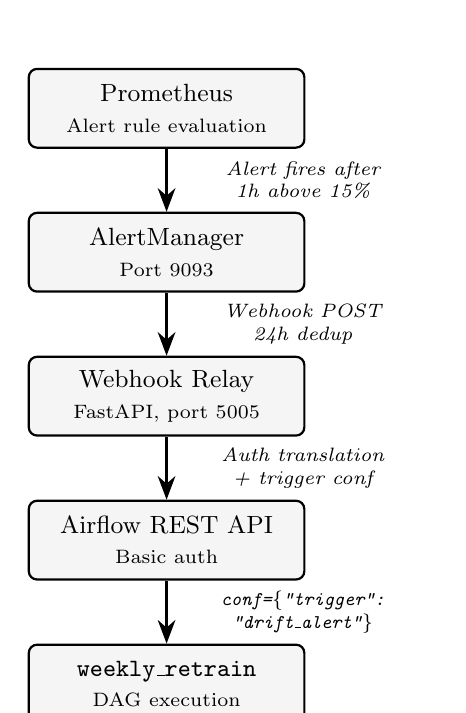
\begin{tikzpicture}[
    node distance=0.8cm,
    block/.style={draw, rectangle, rounded corners=3pt, fill=gray!8,
                  minimum width=3.5cm, minimum height=1cm,
                  font=\small, align=center, thick},
    arrow/.style={-{Stealth[length=3mm]}, thick},
    note/.style={font=\scriptsize\itshape, text width=3.2cm, align=center}
]

% Nodes
\node[block] (prom) {Prometheus\\{\scriptsize Alert rule evaluation}};
\node[block, below=of prom] (am) {AlertManager\\{\scriptsize Port 9093}};
\node[block, below=of am] (webhook) {Webhook Relay\\{\scriptsize FastAPI, port 5005}};
\node[block, below=of webhook] (airflow) {Airflow REST API\\{\scriptsize Basic auth}};
\node[block, below=of airflow] (dag) {\texttt{weekly\_retrain}\\{\scriptsize DAG execution}};

% Arrows with annotations
\draw[arrow] (prom) -- node[right, note] {Alert fires after\\1h above 15\%} (am);
\draw[arrow] (am) -- node[right, note] {Webhook POST\\24h dedup} (webhook);
\draw[arrow] (webhook) -- node[right, note] {Auth translation\\+ trigger conf} (airflow);
\draw[arrow] (airflow) -- node[right, note] {\texttt{conf=\{"trigger":\\"drift\_alert"\}}} (dag);

\end{tikzpicture}
\caption{Drift-triggered retraining chain. The webhook relay exists because
         AlertManager cannot natively authenticate against Airflow's REST
         API.}
\label{fig:drift-chain}
\end{figure}

The 15\% threshold and one-hour window were chosen empirically: under
normal operation with the current synthetic data, fewer than 5\% of events
exceed T1. A sustained elevation above 15\% indicates that the score
distribution has shifted materially, not that a single burst of legitimate
anomalies occurred.


\subsection{Feedback-Triggered Retraining}

The third trigger is described in Section~\ref{sec:feedback-loop}, as it
depends on the supervisor feedback mechanism.


% ═══════════════════════════════════════════════════════════
\section{Supervisor Feedback Loop}
\label{sec:feedback-loop}
% ═══════════════════════════════════════════════════════════

The feedback loop is the single human touch point in the MLOps lifecycle.
When the streaming pipeline produces an alert at the ALERT or BLOCK tier,
the branch supervisor reviews it in the dashboard
(Chapter~\ref{ch:dashboard}) and either confirms or rejects it. This
decision is submitted to the simulation API via a
\texttt{POST /api/v1/feedback} endpoint, which writes the supervisor's
verdict to the \texttt{evaluation\_labels} table in PostgreSQL with a
safe foreign key reference to the original transaction.

These labels serve two purposes. First, they provide ground truth for
evaluating model performance on real decisions --- a capability that
becomes meaningful once the system operates on real transaction data
rather than synthetic events with oracle labels. Second, they feed the
feedback divergence DAG.

\subsection{Feedback Divergence DAG}

An Airflow DAG (\texttt{dags/feedback\_monitor.py}) runs daily and executes
a SQL query against the \texttt{evaluation\_labels} table: over a rolling
seven-day window, what fraction of ALERT and BLOCK tier events were
rejected by supervisors? If the rejection rate exceeds 50\% with a minimum
of 10 reviewed events, the DAG triggers the \texttt{weekly\_retrain} DAG
with \texttt{conf=\{"trigger": "feedback\_divergence"\}}.

The 50\% threshold reflects a simple principle: if more than half of the
system's high-confidence alerts are being overridden by human reviewers,
the models are producing more noise than signal at the upper tiers and
should be retrained. The minimum of 10 reviews prevents a single rejected
alert early in a deployment from triggering an unnecessary retraining
cycle.

\subsection{Three Triggers, One Pipeline}

Table~\ref{tab:retrain-triggers} summarizes the three retraining paths.

\begin{table}[H]
\centering
\caption{Retraining trigger comparison}
\label{tab:retrain-triggers}
\begin{tabular}{@{}llll@{}}
\toprule
\textbf{Trigger} & \textbf{Source} & \textbf{Condition} & \textbf{Frequency} \\
\midrule
Scheduled    & Airflow cron        & Weekly              & Fixed \\
Drift        & Prometheus alert    & $>$15\% above T1 for 1h & On demand \\
Feedback     & Supervisor reviews  & $>$50\% rejection, $\geq$10 reviews & Daily check \\
\bottomrule
\end{tabular}
\end{table}

All three paths converge on the same \texttt{weekly\_retrain} DAG. The
\texttt{conf} parameter passed at trigger time records which path initiated
the run, providing traceability in the Airflow logs without requiring
separate DAG definitions for each trigger type.


% ═══════════════════════════════════════════════════════════
\section{Observability and Monitoring}
\label{sec:observability}
% ═══════════════════════════════════════════════════════════

Observability covers two complementary concerns: \textit{metrics} for
real-time dashboarding and alerting, and \textit{logs} for post-incident
diagnosis.

\subsection{Service Metrics}

Each streaming service (enrichment, scoring, decision) embeds a
\texttt{ServiceMetrics} class from \texttt{src/monitoring/metrics.py} that
exposes two Prometheus instruments:

\begin{itemize}
    \item A \textbf{Counter} tracking the total number of events processed,
          labeled by service name and outcome (success or error).
    \item A \textbf{Histogram} measuring per-event processing latency in
          seconds, enabling percentile queries (p50, p95, p99) in Grafana.
\end{itemize}

Each service exposes its metrics on a dedicated port: enrichment on 9100,
scoring on 9101, and decision on 9102. A Kafka exporter container (port
9308) provides broker-level metrics including consumer group lag --- the
difference between the latest produced offset and the latest committed
offset --- which serves as the primary indicator of pipeline backpressure.
Prometheus scrapes all four targets at a configurable interval
(\texttt{config/prometheus.yml}).

\subsection{Failure Domain Separation}

A monitoring system must not share a failure domain with the service it
monitors. If the enrichment service and its health reporter both depend on
Redis, a Redis outage would simultaneously break the service \textit{and}
suppress the alert that should report the breakage. This principle ruled
out Redis-based heartbeat mechanisms early in the design process.

The chosen architecture avoids this problem: Prometheus pulls metrics over
HTTP from each service's embedded metrics endpoint. The only shared
dependency is the network layer itself, which is an acceptable residual
risk --- if the network is down, no monitoring architecture can report it
from within the affected network.

\subsection{Structured Logging}

All streaming services use a \texttt{JsonFormatter} class
(\texttt{src/streaming/logger.py}) that outputs one JSON object per log
line. Each line includes a timestamp, service name, log level, and message,
with optional contextual fields such as \texttt{event\_id},
\texttt{client\_id}, and \texttt{error\_type} attached as structured
extras.

A \texttt{setup\_logger(service\_name)} factory configures Python's
standard \texttt{logging} module with the JSON formatter, replacing all
\texttt{print()} statements that existed in earlier versions of the
codebase. Structured JSON logs enable downstream processing --- filtering
by service, grouping by error type, or correlating events across services
by \texttt{event\_id} --- without fragile regular expression parsing of
human-readable log strings.

% --- Chapter 7 ---
\chapter{Dashboard and Results}
\label{ch:dashboard}
This chapter describes the supervisor-facing interface and presents the
end-to-end validation results of the complete system.

% ═══════════════════════════════════════════════════════════
\section{Dashboard Architecture}
\label{sec:dashboard-arch}
% ═══════════════════════════════════════════════════════════

The Streamlit dashboard is the only component the branch supervisor
interacts with directly. Every other service --- RedPanda, Redis, the
scoring pipeline --- is invisible infrastructure. The dashboard must
therefore surface the right information clearly while remaining responsive
under continuous use.

\subsection{Why the Dashboard Cannot Consume Kafka Directly}

Streamlit's execution model re-runs the entire Python script from top to
bottom on every user interaction: clicking a button, changing a filter, or
navigating between pages triggers a full re-execution. A Kafka consumer
embedded in the script would be destroyed and recreated on each interaction,
losing its consumer group offset and replaying messages from the last
committed position. This makes direct Kafka consumption architecturally
incompatible with Streamlit.

The solution is the sink consumer pattern described in
Chapter~\ref{ch:streaming}: two independent consumers write streaming
results to PostgreSQL (the \texttt{alerts} table) and Redis (risk history)
continuously. The dashboard reads from PostgreSQL, which provides stable,
queryable, filterable access to all historical alerts without the
limitations of a streaming consumer.

\subsection{Data Access Pattern}

Reads come directly from PostgreSQL using \texttt{psycopg2} with
Streamlit's \texttt{@st.cache\_data} decorator for query-level caching.
Cache TTLs are tuned per page: 10 seconds for the alerts list (where
freshness matters) and 30 seconds for KPI aggregations (where stability
matters more than immediacy).

A \texttt{safe\_query()} wrapper in \texttt{src/dashboard/db.py} handles
connection resilience. If a query fails due to a stale connection --- common
after Docker restarts or idle timeouts --- the wrapper clears the cached
connection, establishes a new one, and retries the query transparently. This
single-retry pattern avoids the complexity of a connection pool while
handling the most common failure mode.

Writes go exclusively through FastAPI endpoints. The dashboard never
executes \texttt{INSERT} or \texttt{UPDATE} statements against the database.
This preserves the single-writer principle and ensures that all write-path
logic --- validation, audit logging, the feedback loop --- lives in one
place.

\subsection{Real-Time Refresh}

The \texttt{streamlit-autorefresh} component triggers a page re-execution
every 10 seconds. Streamlit does not support native WebSocket push from
server to client, so periodic polling is the pragmatic alternative. The
10-second interval balances responsiveness (a new BLOCK-tier alert appears
within 10 seconds of being written to PostgreSQL) against unnecessary
database load from overly aggressive polling.

\subsection{Navigation Structure}

The dashboard uses Streamlit's multi-page application structure, where each
page is an independent Python file in a \texttt{pages/} directory. Navigating
to a page executes only that page's script, avoiding the overhead of loading
data for all pages on every interaction. A shared \texttt{components.py}
module renders the sidebar on every page, displaying pipeline status
indicators and pending alert counts grouped by tier.


% ═══════════════════════════════════════════════════════════
\section{Alerts Page}
\label{sec:dashboard-alerts}
% ═══════════════════════════════════════════════════════════

The alerts page is the supervisor's primary workspace. It presents a
filterable list of alerts with expandable detail for each entry.

\subsection{Filtering and List View}

The supervisor can filter alerts by tier (BLOCK, ALERT, REVIEW), operation
type (retrait, versement, virement, cheque), and review status (pending,
confirmed, rejected). Each alert row displays a color-coded tier badge,
operation type, transaction amount, timestamp, fused anomaly score, and
current review status.

\subsection{Alert Detail}

Expanding an alert reveals the full context needed for a supervisory
decision: client, employee, and branch identifiers; the triggered rules
from the Decision Service with their descriptions; any regulatory flags
with warning icons; and the SHAP explanation.

The SHAP explanation is presented in two layers. The first layer displays
the human-readable narrative generated by the deterministic NLG templates
described in Chapter~\ref{ch:training} --- sentences such as ``This
versement is flagged because the amount is 4.2 times the client's 30-day
average and it is the third deposit within 48 hours.'' The second layer,
hidden behind an expandable section, shows the raw feature-level
contributions: per-feature SHAP values for the Autoencoder and
expected-versus-actual deviations for the LSTM. This two-layer design
serves both audiences: supervisors who need a quick justification and
analysts who want to understand the model's internal reasoning.

\subsection{Supervisor Feedback}

Each pending alert presents two buttons: \textbf{Confirm} and
\textbf{Reject}, with an optional comment field. Clicking either button
sends a \texttt{POST} request to the \texttt{/api/v1/feedback} endpoint
on the FastAPI simulation API, which updates the \texttt{supervisor\_decision}
and \texttt{decision\_timestamp} columns in the \texttt{alerts} table and
upserts a corresponding record into the \texttt{evaluation\_labels} table.
The page then clears its cache and re-renders immediately, reflecting the
updated status without waiting for the next autorefresh cycle.


% ═══════════════════════════════════════════════════════════
\section{KPIs Page}
\label{sec:dashboard-kpis}
% ═══════════════════════════════════════════════════════════

The KPIs page provides an aggregated view of system activity for
operational oversight. Four metric cards at the top display the total
alert count and the count for each of the three actionable tiers (BLOCK,
ALERT, REVIEW). Below the cards, four Plotly charts visualize different
dimensions of the alert data:

\begin{itemize}
    \item A \textbf{pie chart} showing the distribution of alerts across
          tiers, giving an immediate sense of how frequently the system
          escalates to high-severity classifications.
    \item A \textbf{bar chart} grouped by operation type, revealing which
          of the four caisse operations generates the most alerts.
    \item A \textbf{line chart} of alerts per day over the simulation
          period, useful for identifying temporal patterns or spikes.
    \item A \textbf{bar chart} of the top 20 branches by alert count,
          highlighting branches that may warrant closer supervisory
          attention.
\end{itemize}

All aggregation queries use a 30-second cache TTL, trading a small
amount of staleness for reduced database load when multiple supervisors
access the page concurrently.


% ═══════════════════════════════════════════════════════════
\section{Simulation Page}
\label{sec:dashboard-simulation}
% ═══════════════════════════════════════════════════════════

The simulation page allows a supervisor to manually construct a
hypothetical transaction and submit it for scoring without injecting it
into the live pipeline. This serves two purposes: testing whether a
suspicious transaction would trigger an alert before it is processed, and
training supervisors to understand how the system evaluates different
transaction profiles.

The input form collects client ID, employee ID, transaction amount,
operation type, and conditional payload fields (beneficiary ID for
virements, emitter ID and cheque number for cheques). Client-side
validation checks for required fields, positive amounts, and payload
consistency before the form is submitted. The form sends a \texttt{POST}
request to the \texttt{/api/v1/score} endpoint, which runs the full
scoring pipeline synchronously --- enrichment, AE and LSTM inference,
score fusion, SHAP explanation, and decision rules --- and returns the
result.

The response is displayed as a color-coded tier badge, the fused anomaly
score, any triggered rules and regulatory flags, and the full SHAP
explanation in the same two-layer format used on the alerts page.


% ═══════════════════════════════════════════════════════════
\section{Health Page}
\label{sec:dashboard-health}
% ═══════════════════════════════════════════════════════════

The health page queries the Prometheus HTTP API to display the operational
status of the streaming pipeline. Six service status indicators show
whether each service is reachable: the three core streaming services
(enrichment, scoring, decision), the two sink consumers (raw-events sink,
decisions sink), and the simulation API. Each indicator queries the
Prometheus \texttt{up} metric for the corresponding scrape target and
displays a green or red badge.

Below the status indicators, the page displays three operational metrics
derived from the Prometheus instruments described in
Section~\ref{sec:observability}: throughput (events processed per second,
computed from the Counter's rate), p95 processing latency (from the
Histogram), and consumer lag per topic partition (from the Kafka exporter).
If Prometheus is unreachable, the page degrades gracefully to a warning
message rather than crashing, since a monitoring outage should not prevent
the supervisor from accessing other dashboard pages.


% ═══════════════════════════════════════════════════════════
\section{Pipeline Validation and Results}
\label{sec:results}
% ═══════════════════════════════════════════════════════════

With all components integrated --- synthetic data generator, streaming
pipeline, batch profiles, ML models, decision rules, sink consumers, and
dashboard --- the system was validated end-to-end by replaying the full
243,000-event synthetic dataset through the streaming pipeline and
observing the resulting alert distribution.

\subsection{Score Distribution}

Table~\ref{tab:tier-distribution} shows the tier distribution produced by
the validated pipeline after resolving the cold-start and buffer
duplication issues described in Chapter~\ref{ch:streaming}.

\begin{table}[H]
\centering
\caption{Alert tier distribution on the synthetic dataset}
\label{tab:tier-distribution}
\begin{tabular}{@{}lrr@{}}
\toprule
\textbf{Tier} & \textbf{Proportion} & \textbf{Interpretation} \\
\midrule
INFO   & 89\%   & Normal operations, no action required \\
REVIEW & 11\%   & Mild deviations, logged for audit \\
ALERT  & 0.35\% & Significant anomalies, supervisor review \\
BLOCK  & $<$0.1\% & High-confidence anomalies, immediate action \\
\bottomrule
\end{tabular}
\end{table}

The score range spans from 0.015 (routine transactions by established
clients) to 0.999 (high-confidence anomalies matching multiple detection
mechanisms). The distribution is heavily right-skewed, with the vast
majority of events scoring well below the T1 threshold of 0.95. This
shape is expected: in a functioning anomaly detection system, most
transactions should be normal, and the alert tiers should form a steep
pyramid with very few events at the top.

\subsection{Model Performance}

Table~\ref{tab:model-auc} reports the AUC-ROC scores for both models
after retraining on the 30-feature schema.

\begin{table}[H]
\centering
\caption{Model AUC-ROC on the 30-feature schema}
\label{tab:model-auc}
\begin{tabular}{@{}lrr@{}}
\toprule
\textbf{Model} & \textbf{AUC (74 features)} & \textbf{AUC (30 features)} \\
\midrule
Autoencoder & 0.9853 & 0.9714 \\
LSTM        & 0.9866 & 0.9355 \\
\bottomrule
\end{tabular}
\end{table}

The AUC decrease after the feature reduction is expected. The 74-feature
schema included raw profile statistics that made anomalies trivially
separable --- a client whose \texttt{tx\_count\_30d} is zero but who
suddenly transacts is obvious to any model. The 30-feature contrast schema
forces the models to detect anomalies from relative deviations rather than
absolute values, which is harder but more generalizable: the same contrast
features work across archetypes without archetype-specific thresholds.

The LSTM loses more than the Autoencoder because it operates on sequences
of 30-dimensional feature vectors rather than individual events. Each step
in the sequence carries less information per dimension, reducing the LSTM's
ability to model fine-grained temporal patterns. Despite this, both models
remain well above the 0.90 AUC threshold that would indicate reliable
discrimination.

\subsection{Synthetic Data Caveat}

These results validate the system's ability to learn patterns, serve
predictions at streaming latency, and produce a realistic alert
distribution --- but they are not a production performance benchmark. The
synthetic data generator produces anomalies according to known scenarios
with known parameters. Real-world anomalies are messier, more diverse,
and not drawn from the same distribution.

The engineering argument is different from the statistical one: the system
is designed so that plugging in real transaction data requires no code
changes. The generator is replaced by real event sources; the batch
pipeline rebuilds profiles from real history; the models are retrained on
real features computed by the same \texttt{\_compute\_features()} function;
and the retraining triggers (Chapter~\ref{ch:mlops}) ensure that the
models adapt as the data distribution evolves. The AUCs reported here
confirm that this pipeline works end-to-end, not that it will achieve the
same numbers on production data.


% --- Chapter 8 ---
\chapter{Production Roadmap }
\label{ch:roadmap}
This chapter documents the enhancements that would be required to transition
the platform from its current Docker Compose deployment to a
production-grade banking environment.

% ═══════════════════════════════════════════════════════════
\section{Container Orchestration with Kubernetes}
\label{sec:kubernetes}
% ═══════════════════════════════════════════════════════════

The current deployment runs 20 Docker Compose services on a single host.
This is sufficient for development and demonstration, but a production
deployment requires horizontal scaling, automatic failover, and
resource-aware scheduling across multiple nodes.

Kubernetes would replace Docker Compose as the orchestration layer. Each
streaming service (enrichment, scoring, decision) would run as a Deployment
with configurable replica counts, allowing the system to scale horizontally
under increased transaction volume. Health checks already exposed by the
Prometheus metrics endpoints can serve as Kubernetes liveness and readiness
probes with no code changes. The model volume mount --- currently a shared
Docker volume --- would migrate to a Persistent Volume Claim, preserving
the retrain-without-rebuild pattern established in
Chapter~\ref{ch:mlops}.

RedPanda, Redis, and PostgreSQL would each run as StatefulSets with
persistent storage, or be replaced by managed cloud equivalents depending
on the bank's infrastructure policy.


% ═══════════════════════════════════════════════════════════
\section{Continuous Integration and Deployment}
\label{sec:cicd}
% ═══════════════════════════════════════════════════════════

The project currently has no automated CI/CD pipeline. Code changes are
tested manually and deployed by rebuilding Docker images. A production
pipeline would introduce three stages:

\begin{enumerate}
    \item \textbf{Continuous Integration} --- on every commit, run unit
          tests for the three core modules (EnrichmentCore, ScoringCore,
          DecisionCore), validate that the feature computation produces
          the expected 30-dimensional output, and lint the codebase.
    \item \textbf{Image Build} --- on merge to the main branch, build and
          tag Docker images for each service with the commit hash,
          ensuring traceability between deployed code and source control.
    \item \textbf{Staged Deployment} --- deploy to a staging environment
          first, run the E2E test script against the staging pipeline,
          and promote to production only after validation passes.
\end{enumerate}

The core extraction pattern (Chapter~\ref{ch:streaming}) simplifies CI
significantly: the pure core modules can be unit-tested without Redis,
PostgreSQL, or RedPanda dependencies, covering the majority of the
business logic with fast, isolated tests.


% ═══════════════════════════════════════════════════════════
\section{Secrets Management}
\label{sec:secrets}
% ═══════════════════════════════════════════════════════════

Database credentials, API keys, and the Airflow REST API password are
currently stored in a \texttt{.env} file excluded from version control
via \texttt{.gitignore}. This is adequate for a single-developer
environment but insufficient for production, where secrets must be
rotated, audited, and never stored on disk in plaintext.

A secrets management solution such as HashiCorp Vault or cloud-native
equivalents (AWS Secrets Manager, Azure Key Vault) would provide
encrypted storage, automatic rotation, and access logging. Docker Compose
secrets or Kubernetes Secrets would inject credentials at runtime,
eliminating environment files entirely.


% ═══════════════════════════════════════════════════════════
\section{Load Testing}
\label{sec:load-testing}
% ═══════════════════════════════════════════════════════════

The system has been validated with the synthetic dataset of 243,000 events
replayed at accelerated speed, but it has not been tested under sustained
production-equivalent load. A load testing phase would establish the
throughput ceiling of each service, identify the first bottleneck in the
pipeline, and determine the point at which consumer lag begins to
accumulate.

The existing event simulator can serve as the load generator with minimal
modification: adjusting the inter-event delay to simulate peak branch
hours across 150 branches. The Prometheus instrumentation
(Section~\ref{sec:observability}) already captures the metrics needed to
evaluate load test results --- throughput, p95 latency, and consumer lag
--- without additional tooling.


% ═══════════════════════════════════════════════════════════
\section{Data Retention and Archival}
\label{sec:data-retention}
% ═══════════════════════════════════════════════════════════

The current PostgreSQL schema retains all transactions and alerts
indefinitely. In a production deployment, regulatory requirements and
storage constraints necessitate a data retention policy. Tunisian banking
regulations require that transaction records be preserved for a minimum
period, after which they may be archived to cold storage or purged.

A retention strategy would partition the \texttt{transactions} and
\texttt{alerts} tables by month using PostgreSQL's native table
partitioning, enabling efficient archival of older partitions to
compressed cold storage while keeping recent data queryable at full
speed. The batch profile rebuild
(Chapter~\ref{ch:streaming}) would be scoped to the retention window
rather than the full transaction history, reducing nightly computation
time as the dataset grows.

% --- General Conclusion ---
\chapter*{General Conclusion}
\addcontentsline{toc}{chapter}{General Conclusion}
This internship project set out to design and build a real-time anomaly
detection platform for branch teller operations at Amen Bank, covering
four operation types: retrait, versement, virement, and remise de
chèques. The result is a working end-to-end system that ingests
transaction events, computes behavioral features, scores them with two
complementary deep learning models, applies regulatory rules, and
surfaces explainable alerts to branch supervisors through an interactive
dashboard.

The platform monitors two independent actors --- the client initiating
the transaction and the employee processing it --- reflecting the
dual-actor nature of branch teller operations where anomalies can
originate from either side. A streaming architecture built on RedPanda
chains four microservices through message topics, supported by a
hot/cold data layer (Redis and PostgreSQL) and a batch pipeline for
nightly profile reconstruction. The Autoencoder detects point anomalies
in individual transactions while the LSTM identifies sequential
deviations in client behavior over time, with a sigmoid-weighted fusion
mechanism that adapts to account maturity. Every alert carries a
human-readable SHAP explanation generated by deterministic templates,
enabling supervisors to understand and act on the system's output
without requiring machine learning expertise.

Beyond the detection pipeline, the project invested heavily in the
infrastructure that makes a machine learning system maintainable. MLflow
tracks every training experiment. An automated promotion gate ensures
that only models matching or exceeding current production performance
are deployed. Three independent retraining triggers --- a weekly
schedule, a Prometheus-driven drift detector, and a supervisor feedback
divergence monitor --- close the loop between model serving and model
improvement. Structured JSON logging, Prometheus metrics, and Grafana
dashboards provide the observability layer needed to diagnose issues
without inspecting individual events.

The system was validated on a synthetic dataset of 243,000 events
generated from five client archetypes calibrated against Amen Bank's
published data. The validation confirms that the pipeline works
end-to-end --- from event ingestion to supervisor alert --- and that
the retraining subsystem can detect drift and trigger model updates
autonomously. The synthetic data caveat is explicit: these results
demonstrate engineering readiness, not production-grade detection
accuracy. The architecture is designed so that replacing synthetic
data with real transactions requires no code changes --- the same
feature computation, the same models, and the same retraining
pipeline apply without modification.

This project provided the opportunity to work across the full spectrum
of a machine learning system: from data engineering and model training
to streaming infrastructure, MLOps, and front-end delivery. The most
valuable lesson was that building a model is a small fraction of the
effort --- the majority of the engineering work lies in the
infrastructure that ensures the model remains correct, observable, and
improvable over time.


\begin{thebibliography}{99}

\bibitem{bolton2002}
R.~J. Bolton and D.~J. Hand,
``Statistical Fraud Detection: A Review,''
\textit{Statistical Science}, vol.~17, no.~3, pp.~235--255, 2002.

\bibitem{liu2008}
F.~T. Liu, K.~M. Ting, and Z.-H. Zhou,
``Isolation Forest,''
in \textit{Proc. IEEE Int. Conf. Data Mining (ICDM)}, pp.~413--422, 2008.

\bibitem{breunig2000}
M.~M. Breunig, H.-P. Kriegel, R.~T. Ng, and J.~Sander,
``LOF: Identifying Density-Based Local Outliers,''
in \textit{Proc. ACM SIGMOD}, pp.~93--104, 2000.

\bibitem{sakurada2014}
M.~Sakurada and T.~Yairi,
``Anomaly Detection Using Autoencoders with Nonlinear Dimensionality Reduction,''
in \textit{Proc. MLSDA Workshop}, pp.~4--11, 2014.

\bibitem{an2015}
J.~An and S.~Cho,
``Variational Autoencoder based Anomaly Detection using Reconstruction Probability,''
\textit{SNU Data Mining Center, Special Lecture on IE}, 2015.

\bibitem{hochreiter1997}
S.~Hochreiter and J.~Schmidhuber,
``Long Short-Term Memory,''
\textit{Neural Computation}, vol.~9, no.~8, pp.~1735--1780, 1997.

\bibitem{bontemps2016}
L.~Bontemps, J.~McDermott, and N.-A. Le-Khac,
``Collective Anomaly Detection based on Long Short-Term Memory Recurrent Neural Networks,''
in \textit{Proc. Int. Conf. Digital Forensics and Cyber Crime (ICDF2C)}, pp.~141--152, 2016.

\bibitem{aggarwal2017}
C.~C. Aggarwal,
\textit{Outlier Analysis}, 2nd ed.
Springer, 2017.

\bibitem{lundberg2017}
S.~M. Lundberg and S.-I. Lee,
``A Unified Approach to Interpreting Model Predictions,''
in \textit{Advances in Neural Information Processing Systems (NeurIPS)}, pp.~4765--4774, 2017.

\bibitem{kreps2011}
J.~Kreps, N.~Narkhede, and J.~Rao,
``Kafka: A Distributed Messaging System for Log Processing,''
in \textit{Proc. NetDB Workshop}, 2011.

\end{thebibliography}
% ============================================================
% ANNEXES
% ============================================================
\appendix
\chapter{Enriched Feature Schema}
This appendix lists the 30 enriched features computed by the Enrichment
Service for each transaction event. These features constitute the input
vector for both the Autoencoder and the LSTM models.

\begin{longtable}{@{}rllp{6.5cm}@{}}
\caption{Complete enriched feature schema (30 features)}
\label{tab:full-feature-schema} \\
\toprule
\textbf{\#} & \textbf{Feature} & \textbf{Category} & \textbf{Description} \\
\midrule
\endfirsthead
\toprule
\textbf{\#} & \textbf{Feature} & \textbf{Category} & \textbf{Description} \\
\midrule
\endhead
\midrule
\multicolumn{4}{r}{\textit{Continued on next page}} \\
\endfoot
\bottomrule
\endlastfoot

1  & \texttt{amount}                     & Raw event & Transaction amount in DT \\
2  & \texttt{hour}                       & Raw event & Hour of day (0--23) \\
3  & \texttt{is\_retrait}                & Raw event & One-hot: operation is retrait \\
4  & \texttt{is\_versement}              & Raw event & One-hot: operation is versement \\
5  & \texttt{is\_virement}               & Raw event & One-hot: operation is virement \\
6  & \texttt{is\_cheque}                 & Raw event & One-hot: operation is remise de chèques \\
7  & \texttt{is\_home\_branch}           & Raw event & 1 if transaction at client's home branch \\
\midrule

8  & \texttt{z\_amount}                  & Amount contrast & $(x - \mu_{30d}) / \sigma_{30d}$ for this operation type \\
9  & \texttt{amount\_to\_mean\_ratio}    & Amount contrast & $x / \mu_{30d}$ for this operation type \\
10 & \texttt{is\_above\_threshold}       & Amount contrast & 1 if amount $\geq$ 10{,}000 DT \\
11 & \texttt{is\_near\_threshold}        & Amount contrast & 1 if amount $\in$ [8{,}000, 9{,}999] DT \\
12 & \texttt{is\_round\_amount}          & Amount contrast & 1 if amount mod 1{,}000 $=$ 0 \\
13 & \texttt{is\_near\_cheque\_ceiling}  & Amount contrast & 1 if cheque amount $\in$ [25{,}000, 29{,}999] DT \\
\midrule

14 & \texttt{op\_type\_probability}      & Operation contrast & Client's 30d frequency ratio for this operation type \\
\midrule

15 & \texttt{is\_outside\_hours}         & Timing contrast & 1 if hour $\notin$ [8, 16] \\
16 & \texttt{day\_distance\_from\_preferred} & Timing contrast & $|$day of month $-$ client's preferred day$|$ \\
\midrule

17 & \texttt{is\_new\_counterparty}      & Counterparty contrast & 1 if beneficiary/emitter not in known set \\
\midrule

18 & \texttt{tx\_count\_24h}             & Velocity & Client transactions in last 24 hours \\
19 & \texttt{tx\_count\_7d}              & Velocity & Client transactions in last 7 days \\
20 & \texttt{cumulative\_amount\_24h}    & Velocity & Sum of client amounts in last 24 hours \\
21 & \texttt{has\_duplicate\_recent}     & Velocity & 1 if same amount + operation in last 24h \\
22 & \texttt{near\_threshold\_count\_7d} & Velocity & Events in [8k, 10k) DT band in last 7 days \\
\midrule

23 & \texttt{employee\_tx\_count\_24h}          & Employee & Employee's transaction count in last 24h \\
24 & \texttt{same\_employee\_client\_count\_24h} & Employee & Times this employee served this client in 24h \\
\midrule

25 & \texttt{is\_salaried}               & Context & One-hot: archetype is salaried \\
26 & \texttt{is\_small\_business}        & Context & One-hot: archetype is small business \\
27 & \texttt{is\_student}                & Context & One-hot: archetype is student \\
28 & \texttt{is\_retiree}                & Context & One-hot: archetype is retiree \\
29 & \texttt{is\_big\_business}          & Context & One-hot: archetype is big business \\
30 & \texttt{account\_age\_days}         & Context & Days since account opening \\

\end{longtable}

Features 8--9 use a three-level fallback chain when statistics are
unavailable for the current operation type: 30-day statistics, then
90-day statistics, then the archetype baseline. Feature~13 applies only
to cheque operations and is zero for all other operation types.
Features~18--22 are computed from the Redis rolling buffer, not from the
PostgreSQL profile, ensuring they reflect the most recent events with
sub-second latency.

\chapter{Docker Compose Service Inventory}
This appendix lists all 20 Docker Compose services that constitute the
deployed system.

\begin{longtable}{@{}llcp{5cm}@{}}
\caption{Docker Compose service inventory}
\label{tab:docker-services} \\
\toprule
\textbf{Service} & \textbf{Image / Build} & \textbf{Port} & \textbf{Role} \\
\midrule
\endfirsthead
\toprule
\textbf{Service} & \textbf{Image / Build} & \textbf{Port} & \textbf{Role} \\
\midrule
\endhead
\midrule
\multicolumn{4}{r}{\textit{Continued on next page}} \\
\endfoot
\bottomrule
\endlastfoot

\multicolumn{4}{l}{\textit{Infrastructure}} \\
\midrule
redpanda          & vectorized/redpanda      & 9092  & Kafka-compatible message broker \\
redis             & redis:7                  & 6379  & Hot profile store and sequence buffers \\
postgres          & postgres:17              & 5432  & Cold store, alerts, evaluation labels, Airflow metadata \\
\midrule

\multicolumn{4}{l}{\textit{Streaming Pipeline}} \\
\midrule
enrichment-service & Custom (Dockerfile.api) & 9100  & Enriches raw events with 30 contrast features \\
scoring-service    & Custom (Dockerfile.api) & 9101  & AE + LSTM inference, score fusion, SHAP \\
decision-service   & Custom (Dockerfile.api) & 9102  & Rule evaluation, tier assignment \\
raw-events-sink    & Custom (Dockerfile.api) & ---   & Writes raw events to PostgreSQL \\
decisions-sink     & Custom (Dockerfile.api) & ---   & Writes alerts to PostgreSQL and risk history to Redis \\
\midrule

\multicolumn{4}{l}{\textit{API and Dashboard}} \\
\midrule
simulation-api     & Custom (Dockerfile.api) & 8000  & FastAPI: scoring, feedback, health endpoints \\
dashboard          & Custom (Dockerfile.api) & 8501  & Streamlit supervisor dashboard \\
\midrule

\multicolumn{4}{l}{\textit{Orchestration}} \\
\midrule
airflow-webserver  & Custom (Dockerfile.airflow) & 8080  & Airflow UI and REST API \\
airflow-scheduler  & Custom (Dockerfile.airflow) & ---   & DAG scheduling (LocalExecutor) \\
\midrule

\multicolumn{4}{l}{\textit{MLOps}} \\
\midrule
mlflow             & ghcr.io/mlflow/mlflow   & 5001  & Experiment tracking, artifact store \\
webhook-relay      & Custom (Dockerfile.webhook) & ---  & AlertManager $\rightarrow$ Airflow REST API bridge \\
\midrule

\multicolumn{4}{l}{\textit{Monitoring}} \\
\midrule
prometheus         & prom/prometheus          & 9090  & Metrics collection and alert rule evaluation \\
alertmanager       & prom/alertmanager        & 9093  & Alert deduplication and webhook routing \\
grafana            & grafana/grafana          & 3000  & Metrics visualization dashboards \\
kafka-exporter     & danielqsj/kafka-exporter & 9308  & Broker-level metrics (consumer lag) \\
\midrule

\multicolumn{4}{l}{\textit{On-Demand (profile-gated)}} \\
\midrule
hydrate-redis      & Custom (Dockerfile.api) & ---   & Seeds Redis profiles from PostgreSQL at startup \\
simulator          & Custom (Dockerfile.api) & ---   & Replays synthetic events into RedPanda \\

\end{longtable}

Services are organized into six functional groups. The three streaming
pipeline services and two sink consumers form the real-time processing
chain. Infrastructure services (RedPanda, Redis, PostgreSQL) are shared
across all components. The on-demand services (\texttt{hydrate-redis}
and \texttt{simulator}) run once at startup or on explicit invocation
using Docker Compose profiles, and exit after completion.

All custom services share a common \texttt{Dockerfile.api} base image
except the Airflow containers (\texttt{Dockerfile.airflow}, which
excludes PyTorch to save 2\,GB), the webhook relay
(\texttt{Dockerfile.webhook}, a minimal \texttt{python:3.11-slim} image
at approximately 150\,MB), and the training job (launched by the
DockerOperator using a separate \texttt{amen-anomaly-training:latest}
image not listed here, as it runs transiently during retraining).

\clearpage
\thispagestyle{empty}


\end{document}
